\documentclass[a4paper,12pt,twoside]{book}
\usepackage{tfg}
\usepackage{appendix}
\begin{document}

\pagestyle{empty}
Portada
// TO DO //
\newpage
\chapter*{Agradecimientos}
Agradecimientos
// TO DO //
\newpage
\chapter*{Resumen}
Se realizará una aplicación que permite la organización de visitas a diferentes lugares de
una localidad mediante la creación de rutas entre los mismos. Se implementará un
servicio web en Java bajo el paradigma Rest que sirva de API tanto a la aplicación web
como móvil para el acceso a los datos. Los datos de los lugares y sitios que un usuario
pueda buscar serán obtenidos por el servicio web a través de una fuente externa. Los
usuarios podrán consultar los diferentes lugares que existan en una localidad y
mostrarlos en un mapa, para luego, seleccionar los que el usuario desee visitar. Entre
los lugares que el usuario desea visitar se generará una ruta. En dicha ruta, el usuario
podrá especificar el tiempo de comienzo (día y hora que va estar en esa localidad y que
vaya a comenzar la ruta), el tiempo que desea o estima pasar en cada sitio, el orden en
el que los desea visitar, así como el tipo de desplazamiento que va realizar entre cada
sitio (coche, andando, etc…). La aplicación mostrará el tiempo y la distancia que hay
entre cada lugar, así como el total. De esta forma el usuario podrá saber cuánto tiempo
le llevará el viaje y podrá realizar modificaciones en función de sus necesidades.
Además, en la aplicación se podrán registrar eventos temporales (Ejemplo: Feria
gastronómica – Madrid – 20 de Enero) que se integrarán con los lugares ofrecidos por la
fuente externa y que permitirá al usuario incluirlos en sus rutas (si coincidiese en espacio
y tiempo). Los usuarios podrán compartir sus rutas guardadas con el resto de usuarios y
a mayores, en la aplicación móvil se podrá consultar a tiempo real la realización de la
ruta, mediante el uso de la geolocalización, que permitirá al usuario saber si está
cumpliendo o no sus estimaciones indicadas a la hora de la creación de la ruta.
La aplicación hará uso de la API de Foursquare para el acceso a los datos de lugares y
empleará la API de Google para los cálculos de distancias y tiempos, así como para la
visualización en los
mapas. 
\newpage
\chapter*{Palabras Clave}
// TO DO //
\newpage

\setcounter{page}{1}
\cleardoublepage
\tableofcontents
\cleardoublepage
\listoffigures
\cleardoublepage
\listoftables


\setcounter{page}{1}
\chapter[Introducción]{
  \label{chp:introduccion}
  INTRODUCCIÓN
}
\thispagestyle{numberingStyle}
\pagestyle{numberingStyle}


\section{Contextualización}
Durante las últimas décadas, el turismo ha experimentado un continuo crecimiento que lo ha llegado a convertirse en uno de los sectores económicos más importantes. Por su parte, el éxito de la telefonía móvil y el continuo uso de smartphones en la sociedad, promulga el desarrollo de las aplicaciones móviles, otro sector que continúa en pleno crecimiento. Es entre estos dos sectores donde se engloba el desarrollo de la aplicación.

Se pretende presentar a los usuarios finales una aplicación móvil, fácilmente accesible, que permita ofrecer un servicio que ayude a planificar rutas turísticas en un viaje determinado. La creación y planificación de rutas es el objetivo primordial de la aplicación pero no su única funcionalidad. Los usuarios podrán consultar los diferentes lugares del mundo, con un alto nivel de filtrado, permitiendo obtener lugares de una característica o estilo concreto. También podrán consultar eventos, que tendrán una duración de carácter temporal y estarán formados por un conjunto actividades.

Los lugares ofrecidos al usuario serán obtenidos de la base de datos de Foursquare. Foursquare es un servicio basado en localización nacido en 2009 como una red social donde los usuarios hacían registros y recomendaciones sobre los sitios y lugares que visitaban. Con el paso de los años, la situación de la empresa fue empeorando drásticamente hasta perder la popularidad que había conseguido en sus comienzos. En los últimos años, Foursquare se ha rejuvenecido y ahora es una compañía basada en inteligencia de localización. Posee una base de datos muy amplia y de gran nivel que le permite ofrecer esa información a muchas aplicaciones y empresas, y que también servirá a esta aplicación.

También, se pretenderá otorgar a la aplicación un carácter de red social. Las aplicaciones de redes sociales son uno de los mayores atractivos para los usuarios de aplicaciones, y el número de usuarios que las usan aumentan diariamente. De esta forma, otorgando esta característica a nuestra aplicación, permitiendo compartir y consultar rutas hechas o planificadas por demás usuarios de la aplicación, conseguiremos otorgarle un valor añadido a nuestra aplicación.


\section{Objetivos}
El desarrollo de esta aplicación supone la consecución de los siguientes objetivos.

\begin{itemize}

	\item \textbf{Planificar rutas}. El objetivo principal, crear y planificar rutas. La planificación incluirá poder determinar la ciudad o lugar de destino y las fechas en las que se va a realizar dicho viaje. También incluye la posibilidad de buscar lugares de interés o eventos en determinada ciudad y especificar las diferentes horas que se quiere pasar en cada uno de ellos, así como, calcular las distancias que hay entre cada uno de los lugares o eventos incorporados en cada ruta.
	\item \textbf{Obtención datos externos}. Será necesario poder establecer una comunicación con las fuentes de datos externos que nos permita obtener los lugares y calcular las distancias. Este objetivo también incluye la gestión y almacenamiento de estos datos en nuestra aplicación.
	\item \textbf{Gestionar eventos}. Tiene como objetivo crear, modificar, eliminar y consultar los eventos utilizados por la aplicación. Estos eventos, serán consultados por los usuarios cuando realicen la planificación de sus rutas y podrán incorporarlos en ellas.
	\item \textbf{Gestionar de usuarios}. Se pretende conseguir una completa gestión de usuarios que les permita crear rutas propias y compartirlas con los demás usuarios. También, se pretende ofrecer que un usuario pueda marcar una ruta como privada, de forma que no pueda ser accedida por lo demás.
	\item \textbf{Aplicación móvil}. El objetivo de la aplicación es poder ser usada mediante un smartphone o dispositivo móvil inteligente. En la aplicación móvil se pretende incoporar el uso de mapas, permitiendo una planificación de rutas de manera visual y simulada en el mapa. También, como objetivo secundario, se establece la elaboración de una aplicación web con funcionalidades reducidas con respecto a la aplicación móvil y que también permite la administración remota de los datos almacenados en la aplicación.
	\item \textbf{Datos en tiempo real}. El objetivo es poder obtener los datos de geolocalización reales para el día exacto en que se realice la ruta y consultarlos posteriormente en el mapa de la aplicación. De esta forma, los usuarios podrán comparar la planificación de sus rutas con su ejecución real.
	
\end{itemize}


\section{Estructura de la memoria}
En este apartado se detallará el contenido de la memoria donde se incluirá una pequeña descripción para cada capítulo que la componen.

\begin{itemize}
	\item \textbf{Capitulo 2 - Análisis de alternativas}. Se comentarán y analizarán las aplicaciones existentes en el mercado actual que poseen una finalidad semejante a la desarrolla en este proyecto.  
	\item \textbf{Capitulo 3 - Fundamentos tecnológicos}. Capítulo en el que se describirán cada uno de los elementos y componentes, de carácter tecnológico, que sirvieron para realizar de la aplicación.
	\item \textbf{Capitulo 4 - Metodología}. En este capítulo se detallará la metodología de software empleada y se explicarán sus características.
	\item \textbf{Capitulo 5 - Planificación y costes}. Se realizará la planificación del proyecto y se detallará el coste de cada uno de los elementos que lo componen.
	\item \textbf{Capitulo 6 - Análisis}. Apartado donde se detallarán los requisitos necesarios para realizar la aplicación. Se incluirán los diagramas y especificaciones de los casos de uso definidos.
	\item \textbf{Capitulo 7 - Diseño}. En este capítulo se presentará el diseño elaborado para la realización de la aplicación. Se detallará la arquitectura del sistema y de cada uno de los módulos que forman la aplicación.
	\item \textbf{Capitulo 8 - Implementación}. Se explicará la estructura del proyecto y se mostrarán ejemplos de implementación de algunos módulos de la aplicación.
	\item \textbf{Capitulo 9 - Pruebas}. Se detallarán y explicarán las pruebas realizadas.
	\item \textbf{Capitulo 10 - Conclusiones y trabajo futuro}. Capítulo con las conclusiones finales adquiridas después de realizar el proyecto y con las líneas de trabajo futuro a seguir para la continua mejora de la aplicación.
	\item \textbf{Apéndice A - Diagramas}. Apéndice en el que se incluirán diagramas de la aplicación.
	\item \textbf{Apéndice B - Manual de usuario}. Apéndice en el que se explicará la guía de uso de la aplicación.
\end{itemize}



















\chapter[Análisis de alternativas]{
  \label{chp:analisisdealternativas}
  ANÁLISIS DE ALTERNATIVAS
}
\thispagestyle{numberingStyle}
\pagestyle{numberingStyle}



Antes de comenzar el desarrollo de este proyecto, se realizó un breve estudio de algunas de las aplicaciones, de temática similar, disponibles en el mercado. 

La primera en ser analizada ha sido la propia aplicación de Foursquare que, como se comentó con anterioridad, será la fuente de datos de lugares de la aplicación. La aplicación de Foursquare, tanto en su versión web como móvil, ofrece la posibilidad de buscar lugares, sitios de interés y demás, según diferentes criterios, y que pueden ser guardados por el usuario en lo que la aplicación denomina listas. Sin embargo, Foursquare no permite establecer ningún tipo de planificación ni ruta entre dichos sitios.

Por otra parte, existen numerosas aplicaciones enfocadas principalmente a la planificación de rutas. Una de las más populares es la aplicación móvil Google Trips: Travel Planner, aplicación del grupo Google. Está aplicación ofrece gran nivel de detalle en lo que se refiere a la planificación de viajes y se puede considerar una aplicación todo en uno. Permite crear viajes en función de las reservas remitidas al correo electrónico de Google del usuario, añadir planes de viaje diarios, mostrar información sobre el transporte disponible, ofrecer los diferentes descuentos disponibles a determinados lugares, como pueden ser museos, y demás funcionalidades relacionadas.

En su contra, a la hora de establecer los planes diarios, esta aplicación no permite una completa personalización. El modo de transporte utilizado será escogido por la propia aplicación, siendo este el más eficiente en tiempo. Por otra parte, te recomienda el tiempo a pasar en cada visita en función de la media de los demás usuarios, pero no ofrece la posibilidad de establecer un tiempo específico. Estas limitaciones impiden conocer el tiempo total que empleará el usuario en el plan de ese día, a qué horas debería salir de un determinado sitio para llegar a otro antes de una hora específica, modificar el modo de viaje en función de sus necesidades, y demás.


A mayores de las aplicaciones mencionadas, existe gran variedad, como pueden ser Sygic Travel o Visit a City, que ofrecen una funcionalidad principal similar, la planificación de viajes. Cada una de ellas presenta características diferentes, como pueden ser, la fuente de datos utilizada, el nivel de detalle en la planificación, el número de funcionalidades ofrecidas, etc. Estas características y la manera de cómo ofrecerlas, serán las que hagan únicas a las aplicaciones en el mercado y que harán que los usuarios se decanten por el uso de unas u otras.














\chapter[Fundamentos tecnológicos]{
  \label{chp:fundamentos}
  FUNDAMENTOS TECNOLÓGICOS
}

\thispagestyle{numberingStyle}
\pagestyle{numberingStyle}


\section{Lenguajes utilizados}
\subsection{Java}
Java es un lenguaje de programación de propósito general, concurrente, orientado a objetos. Fue diseñado para tener tan pocas dependencias de implementación como fuera posible tal que permitiera a los desarrolladores escribir el programa una vez y ejecutarlo en cualquier dispositivo sin necesidad de recompilarlo.

Fue originalmente desarrollado por James Gosling, de Sun Microsystems, la cual fue adquirida por la compañía Oracle.

Puede ejecutarse en cualquier máquina virtual Java (JVM) sin importar la arquitectura de la computadora subyacente y su sintaxis deriva en gran medida de lenguajes como C y C++, pero con menos utilidades de bajo nivel.

\subsection{JavaScript}
JavaScript es un lenguaje de programación interpretado, dialecto del estándar ECMAScript, orientado a objetos, basado en prototipos, imperativo, débilmente tipado y dinámico.

Se utiliza principalmente del lado del cliente, implementado como parte de un navegador web, permitiendo mejoras en la interfaz de usuario y páginas web dinámicas.

JavaScript se diseñó con una sintaxis similar a C, aunque adopta nombres y convenciones del lenguaje de programación Java. Sin embargo, Java y JavaScript tienen semánticas y propósitos diferentes.

\subsection{TypeScript}
TypeScript es un lenguaje de programación libre y de código abierto desarrollado y mantenido por Microsoft.

Este lenguaje es un superset del ya conocido JavaScript y que está pensado para grandes proyectos, los cuáles a través de un compilador de TypeScript se traducen a código JavaScript original.

Un aspecto característico de TypeScript es su sistema de tipos. Permite a los desarrolladores definir variables y funciones tipadas sin perder la esencia de JavaScript gracias a una representación estática de los tipos dinámicos. Definir tipos durante el diseño, nos ayudará a evitar errores en tiempo de ejecución.

\subsection{HyperText Markup Language}
HyperText Markup Language, conocido comúnmente por sus siglas, HTML, es un lenguaje de marcado cuya finalidad es la elaboración de páginas web. Define una estructura básica y un código (denominado código HTML) para la definición de contenido de una página web. 

Es un estándar a cargo del World Wide Web Consortium (W3C), organización dedicada a la estandarización de casi todas las tecnologías ligadas a la web.

\subsection{Cascading StyleSheets}
Las hojas de estilo en cascada (o CSS, por sus siglas en inglés) es un lenguaje de diseño gráfico para definir y crear la presentación de un documento estructurado escrito en un lenguaje de marcado. Especifica como se mostrarán por pantalla los denominados elementos HTML.

Junto con HTML y JavaScript, CSS es una tecnología usada por muchos sitios web para crear páginas web visualmente atractivas, interfaces de usuario de aplicaciones web y GUIs para muchas aplicaciones móviles.

Su principal objeto es mantener la separación del contenido del documento de su forma de presentación. Con las hojas de estilo se puede prescindir del uso de formatos de estilo dentro de la propia página HTML, de manera que se pueda modificar el estilo de toda una web modificando un único archivo CSS.




\section{Frameworks, librerías y técnicas de desarrollo}
\subsection{Spring}
Spring es un framework cuya finalidad es facilitar el desarrollo de aplicaciones desarrolladas en Java. Es de código abierto y la primera versión fue elaborada por Rod Johnson. A pesar de que no impone ningún modelo de programación en particular, este framework se ha vuelto popular en la comunidad al ser considerado una alternativa, sustituto, e incluso un complemento a varias APIs de Java EE.

Spring está compuesto de diversos módulos que se pueden agregar a nuestras aplicaciones, permitiendo a los desarrolladores agregar sólo los módulos que vayan usar. El único módulo necesario para trabajar con Spring es el Spring Core puesto que es el que contiene la DI (Inyección de Dependencias) y la configuración de uso de objetos Java.

\subsubsection*{Spring MVC}
Spring MVC es un framework de aplicaciones web basado en el patrón MVC(model-view-controller) y que alberga todas las ventajas del framework de Spring.
	\begin{itemize}
		 \item Separación clara de roles. Cada objeto controlador, validador, formulario, de modelo pueden ser realizados por objetos especializados.
		 \item Configuración potente y directa. Capacidad de configuración que permite una fácil referencia a través de contextos, como por ejemplo, desde controladores web a objetos de negocio.
		 \item Adaptabilidad, flexibilidad y no intrusividad. Definir los métodos de cualquier controlador utilizando las anotaciones de parámetros (como @RequestParam, @RequestHeader, @PathVariable, y más).
		 \item Código de negocio reutilizable. No existe necesidad de duplicación.
	\end{itemize}
	
Spring MVC es, como otros frameworks MVC, basado en solicitud (request-driven). Están diseñados en torno a un Servlet central que sirve las solicitudes a los controladores y ofrece unas funcionalidades que facilitan el desarrollo de las aplicaciones web. Sin embargo, el DispatcherServlet de Spring es más que eso, está completamente integrado con el contenedor Spring IoC y permite hacer uso de las características y funcionalidades de Spring.

\subsubsection*{Spring Security}
Spring Security ofrece exhaustivos servicios de seguridad para las aplicaciones empresariales basadas en Java EE. 
Las dos principales áreas en las que se enfoca Spring Security son la Autenticación y la Autorización, probablemente, los dos temas más relevantes en la seguridad de las aplicaciones.
	\begin{itemize}
		\item Autenticación es el proceso por el que se determina que uno es el que dice ser.
		\item Autorización hace referencia al proceso de determinar qué acción o acciones puede realizar en la aplicación.
	\end{itemize}
	
A nivel de autenticación, Spring Security soporta un amplio rango de modelos de autenticación. La mayoría de estos modelos de autenticación son proporcionados por terceros, o desarrollados por los organismos estándar pertinentes, como Internet Engineering Task Force. A mayores, Spring Security provee su propio conjunto de mecanismos de autenticación y soporta integración de autenticación con diferentes tecnologías


\subsection{Java Persistence API}
Java Persistence API, comúnmente conocida por sus siglas JPA, es la API que describe la gestión de datos relacionales en aplicaciones que utilicen Java. La primera especificación fue lanzada en mayo de 2006 como parte del trabajo del JSR 220.

JPA en sí mismo es solo una especificación, no un producto. Son un conjunto de interfaces que requieren una implementación. Existen implementaciones de JPA de código abierto y comerciales, y cualquier servidor de aplicaciones JAVA EE 5 debe proporcionar soporte para su uso.

El objetivo de esta API es no perder las ventajas de la orientación a objetos al interactuar con una base de datos y permitir usar objetos regulares, comúnmente conocidos como POJOs. 

\subsection{JAX-RS}
JAX-RS es la API de Java para la elaboración de servicios web RESTful que brinda soporte en la creación de servicios web de acuerdo con el patrón arquitectónico REST. Desde la versión 1.1, JAX-RS es una parte oficial de Java EE 6. Una característica notable de ser parte oficial de Java EE es que no es necesaria ninguna configuración para comenzar a utilizar JAX-RS.

Esta API utiliza anotaciones, introducidas en Java SE 5, para simplificar el desarrollo y la implementación de clientes y recursos web. 

De la misma forma que sucedía con JPA, JAX-RS no es más que una especificación, necesita un producto que la implemente. Jersey y RESTEasy son implementaciones de JAX-RS,

\subsection{Thymeleaf}
Thymeleaf es una librería Java que implementa un motor de plantillas válidas para entornos web cómo independientes. Es un software de código abierto creado originalmente por un ingeniero de software español llamado Daniel Fernández. No está hecho ni respaldado por ningún software de ninguna compañía y se ofrece al público de manera totalmente gratuita, tanto en formato binario como en código fuente, bajo licencia Apache.

Su objetivo principal es la creación de plantillas de una manera elegante y con un código bien formateado.

Thymeleaf ofrece una buena integración con Spring MVC a través de su dialecto SpringStandard, pero esta integración con Spring es completamente opcional y el dialecto estándar está destinado a usarse sin Spring.

\subsection{jQuery}
jQuery es una librería multiplataforma de JavaScript, creada incialmente por John Resig. Es un software libre y de código abierto, y posee un doble licenciamiento bajo la licencia MIT y la licencia Pública General de GNU, permitiendo su uso en proyectos libres y privados.

Su objetivo es la realización de funcionalidades basadas en JavaScript de forma rápida y sencilla. Permite realizar recorridos y manipulaciones de documentos HTML, manejar eventos, animaciones y usar AJAX  mucho más simple con una API fácil de usar que funciona en multitud de navegadores.

\subsection{Bootstrap}
Bootstrap es un kit de herramientas de código abierto para desarrollo web junto a HTML, CSS y JS.  

Originalmente creado por un diseñador y desarrollador de Twitter, Bootstrap es uno de los frameworks front-end y proyectos de código abierto más populares en el mundo. Antes de ser un framework de código abierto, Bootstrap era conocido como Twitter Blueprint.

Bootstrap incluye plantillas de diseño basadas en HTML y CSS para tipografías, formularios, botones, tablas,... así como complementos de JavaScript opcionales. También brinda la capacidad de crear fácilmente diseños receptivos.

\subsection{AJAX}
AJAX es una técnica de desarrollo web para crear aplicaciones interactivas. Es una tecnología asíncrona, en el sentido que los datos adicionales solicitados al servidor, se cargan en segundo plano sin inferir con la visualización ni el comportamiento de la página.

La funciones de llamada AJAX se efectúan, normalmente, bajo el lenguaje de programación JavaScript mientras que el acceso a los datos se realiza mediante el objeto JavaScript XMLHttpRequest.

AJAX no constituye una tecnología en sí misma, sino que es un término que engloba a un grupo de éstas que trabajan conjuntamente.

	\begin{itemize}
		\item XHTML (o HTML) y CSS para el diseño que acompaña a la información.
		\item Document Object Model (DOM) accedido con un lenguaje de scripting por parte del usuario, generalmente, JavaScript.
		\item El objeto XMLHttpRequest para intercambiar datos de forma asíncrona con el servidor web.
		\item XML es el formato usado generalmente para la transferencia de datos solicitados al servidor.
	\end{itemize}
	

\section{Herramientas de desarrollo}
\subsection{Eclipse}
Eclipse es una plataforma software compuesto por un conjunto de herramientas de programación de código abierto multiplataforma.

Fue desarrollado originalmente por IBM como el sucesor de su familiar de herramientas VisualAge. Ahora, está siendo desarrollado por la Fundación Eclipse, una organización independiente, sin ánimo de lucro, que fomenta una comunidad de código abierto y un conjunto de productos complementarios.

\subsection{Maven}
Maven es una herramienta de software para la gestión y construcción de proyectos Java creada por Jason van Zyl en 2002 que tiene un modelo de configuración de construcción basado en formato XML.

Maven utiliza un Project Object Model, conocido como POM, para describir el proyecto software a construir, sus dependencias de otros módulos y componentes externos, y el orden de construcción de los elementos.

Una de sus características clave son su disponibilidad para usarse en la red puesto que el motor incluido en su núcleo puede dinámicamente descargar plugins de un repositorio.


\subsection{Git}
Git es un sistema de control de versiones distribuido de código abierto y gratuito diseñado para manejar todo, desde proyectos pequeños a muy grandes, con velocidad y eficiencia.

Originalmente fue diseñado como un motor de sistema de control de versiones de bajo nivel sobre el cual otros podían codificar interfaces frontales. Desde entonces hasta ahora, el núcleo del proyecto Git se ha vuelto un sistema de control de versiones completo, utilizable en forma directa.

Git es fácil de aprender y ofrece un rendimiento increíblemente rápido. Su principal objetivo es llevar el registro de cambios en archivos y coordinar el trabajo que varias personas realizan sobre archivos compartidos.


\subsection{Oracle SQL Developer}
Oracle SQL Developer es un entorno de desarrollo integrado y gratuito que simplifica el desarrollo y la administración de las bases de datos de Oracle, tanto de implementaciones tradicionales como en la nube.

Este software admite productos de Oracle y una grana variedad de complementos de terceros que los usuarios pueden implementar para conectarse a bases de datos que no sean de Oracle.

SQL Developer ofrece un desarrollo completo de extremo a extremo de sus aplicaciones PL / SQL, una hoja de trabajo para ejecutar consultas y scripts, una consola DBA para administración, una interfaz de informes y una solución completa de modelado de datos.



\section{Sistema de gestión de bases de datos}
\subsection{Oracle Database}
Oracle Database es un sistema de gestión de base de datos de tipo objeto-relacional, desarrollado por Oracle Corporation. Es la base de datos más popular para el procesamiento de transacciones el línea (OLTP) y almacenes de datos (Data warehousing).

La tecnología Oracle se encuentra prácticamente en todas las industrias alrededor del mundo y es el proveedor mundial líder de software para administración de información.

El producto Oracle para el sistema de base de datos cuenta con 7 ediciones diferentes de las cuales, una es completamente gratuita.

\section{Servidor de aplicaciones}
\subsection{Apache Tomcat}
Apache Tomcat funciona como un contenedor de servlets desarrollado por Apache Software Foundation. Es un una implementación de código abierto de las tecnologías Java Servlet, JavaServer Pages, Java Expression Language y Java WebSocket. Se publica bajo la versión 2 de Apache License.

Tomcat no es un servidor de aplicaciones, pero puede funcionar como servidor web por sí mismo. Actualmente es usado como servidor web autónomo en entornos con alto nivel de tráfico y alta disponibilidad.

Está escrito en Java, de manera que puede funcionar en cualquier sistema operativo que disponga de la máquina virtual Java.



\section{Otros}
\subsection{Ionic}
Ionic es un completo SDK de código abierto diseñado para el desarrollo de aplicaciones móviles híbridas. La versión original fue lanzada en 2013 y construida sobre AngularJS y Apache Cordova. Las versiones más recientes, conocidas como Ionic 3, están construidas sobre Angular.

Proviene de herramientas y servicios para desarrollar aplicaciones móviles híbridas usando tecnologías web (CSS, HTML,...).

Ionic proviene todas la funcionalidades que se puede encontrar en los SDK de desarrollo de aplicaciones nativas. Las aplicaciones construidas se pueden personalizar en función del uso final, Android o iOS, por ejemplo.

Además del SDK, Ionic también brinda servicios que los desarrolladores pueden usar para habilitar funciones, como la tecnología push, test A/B, construcciones automáticas, etc...

Ionic también proporciona una poderosa interfaz de línea de comandos, lo que permite poder comenzar a desarrollar un proyecto con un simple comando. También permite a los desarrolladores agregar complementos de Cordova.




\chapter[Metodología]{
  \label{chp:metodologia}
  METODOLOGÍA
}
\thispagestyle{numberingStyle}
\pagestyle{numberingStyle}

El Proceso Unificado es un marco de desarrollo software caracterizado por estar dirigido por casos de uso, centrado en la arquitectura y por ser iterativo e incremental.


\section{Características}

Para el desarrollo de este proyecto se ha escogido una metodología basada en el Proceso Unificado. Esta metodología nos permite obtener un producto de alta calidad gracias a su carácter iterativo e incremental. De manera que, en cada ciclo o iteración, el producto es revisado y mejorado.

\subsection{Dirigido por casos de uso}
Un caso de uso es un fragmento de funcionalidad del sistema que proporciona un resultado de valor a un usuario. Los casos de uso modelan los requerimientos funcionales del sistema y todos juntos constituyen el  \textit{modelo de casos de uso}.

Los casos de uso también guían el proceso de desarrollo (diseño, implementación y prueba). Basándose en los casos de uso, los desarrolladores crean una serie de modelos de diseño e implementación que llevan a cabo. De este modo, los casos de uso no son solo una herramienta para especificar los requerimientos e iniciar el proceso de desarrollo, sino que también dirigen su diseño, implementación, pruebas, etc...

\subsection{Centrado en la arquitectura}
La arquitectura de un sistema software se describe mediante diferentes vistas del sistema en construcción. Se define arquitectura como el conjunto de decisiones significativas acerca de la organización de un sistema software, la selección de los elementos estructurales a partir de los cuales se compone el sistema y su composición.

Los casos de uso y la arquitectura están profundamente relacionados. Los casos de uso deben encajar en la arquitectura, y esta a su vez, debe permitir el desarrollo de todos los casos de uso requeridos, actualmente y a futuro.

De tal forma que, el arquitecto software desarrolla la forma o arquitectura a partir de la comprensión de un conjunto reducido de casos de uso fundamentales o críticos.

\subsection{Iterativo e incremental}
Se divide el desarrollo de un proyecto software en partes más pequeñas o mini proyectos. Cada mini proyecto es una iteración que supono un incremento. Las iteraciones hacen referencia a pasos en el flujo de trabajo, y los incrementos, a crecimientos en el producto.

Las iteraciones deben estar controladas de manera que se deben seleccionar y ejecutar de forma planificada. 

En cada iteración los desarrolladores identifican y especifican los casos de uso relevantes y crean un diseño utilizando la arquitectura seleccionada para implementar dichos casos de uso. Si la iteración cumple sus objetivos, se continúa con la próxima, si no, deben revisarse las decisiones previas y probar un nuevo enfoque.

\section{Ciclo de vida}
El Proceso Unificado se repite a lo largo de una serie de ciclos que constituyen la vida de un sistema.


\begin{figure}[!h]

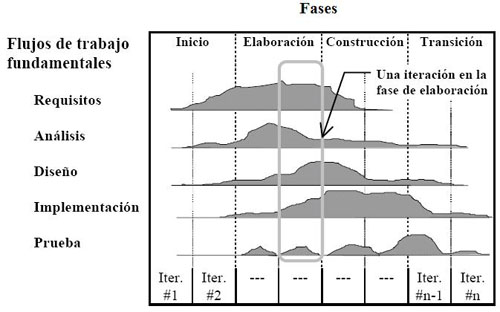
\includegraphics[
   keepaspectratio=true
]{./03_Met_Plan/01_Metodologia/diagramaProcesoUnificado.JPG}
\caption{Ciclo de vida - Proceso Unificado de Desarrollo}
\end{figure}


Cada ciclo consta de cuatro fases: \textbf{Inicio}, \textbf{Elaboración}, \textbf{Construcción} y \textbf{Transición}. Cada fase se divide en iteraciones, en las cuales se desarrolla, secuencialemte, una serie de disciplinas o flujos de trabajo como por ejemplo: \textit{Análisis, Diseño, Implementación y Pruebas.}

En la figura podemos observar que el ciclo de vida del Proceso Unificado presenta dos dimensiones:
\begin{itemize}
	\item Un eje horizontal que representa el aspecto dinámico del proceso conforme se va desarrollando. Expresado en términos de \textit{Fases, Iteraciones e Hitos}.
	\item Un eje vertical que representa el aspecto estático del proceso mediante las disciplinas o flujos de trabajo.
\end{itemize}


\subsection{Fases}

\subsection{Fase de inicio}
Durante la fase de inicio se desarrolla una descripción del producto final y se presenta el análisis de negocio.

El objetivo de esta fase es ayudar al equipo de proyecto a decidir cuales son los verdaderos objetivos del proyecto.

\subsection{Fase de elaboración}
En esta fase se especifican la mayoría de los casos de uso del producto y se diseña la arquitectura del mismo. Se establece una firme comprensión del problema a solucionar.


\subsection{Fase de construcción}
Durante la fase de construcción se elabora el producto, de tal manera que la línea base de la arquitectura avanza hasta convertirse en el sistema completo. Al final de esta fase se obtienen todos los casos de uso implementados aunque pueden incluir defectos.


\subsection{Fase de transición}
La fase de transición hace referencia al período donde el software ya debe estar listo para ser instalado, probado y utilizado. Las iteraciones en esta fase continúan agregando características al software.


\section{Iteraciones}
\subsection{Iteración 1: Análisis de requisitos y diseño}
Planificación\\
Modelado casos de uso\\
Diseño arquitectura

\subsection{Iteración 2: Base inicial del proyecto}
Preparación del entorno\\
Formación en las tecnologías\\
Configuración APIs externas\\
Creación base de datos.

\subsection{Iteración 3: Usuarios}
Analisis y diseño\\
Implementación persistencia\\
Implementación servicios\\
Pruebas

\subsection{Iteración 4: Rutas}
Analisis y diseño\\
Implementación persistencia\\
Implementación servicios\\
Pruebas

\subsection{Iteración 5: Lugares y categorías}
Analisis y diseño\\
Implementación persistencia\\
Implementación servicios\\
Pruebas

\subsection{Iteración 6: Eventos}
Analisis y diseño\\
Implementación persistencia\\
Implementación servicios\\
Pruebas

\subsection{Iteración 7: Servicios externos}
Analisis y diseño\\
Modificación librebría Java Foursquare\\
Implementación servicios\\
Pruebas

\subsection{Iteración 8: Autenticación y Autorización}
Analisis y diseño\\
Formación Json Web Tokens y Spring Security\\
Implementación autenticación\\
Implementación autorización\\
Pruebas

\subsection{Iteración 9: Cliente móvil}
Analisis y diseño\\
Formación IONIC - Angular\\
Implementación acceso a servicios\\
Implementación pantallas y controladores\\
Pruebas

\subsection{Iteración 10: Cliente web}
Analisis y diseño\\
Implementación acceso a servicios\\
Implementación pantallas y controladores\\
Pruebas

\subsection{Iteración 11: Panel de administración}
Analisis y diseño\\
Implementación acceso a servicios\\
Implementación pantallas y controladores\\
Pruebas

\subsection{Iteración 12: Cierre}
Evaluación de la aplicación final y revisión.






\chapter[Planificación y costes]{
  \label{chp:planificacion}
  PLANIFICACIÓN Y COSTES
}
\thispagestyle{numberingStyle}
\pagestyle{numberingStyle}



\section{Planificación}

\subsection{División de las tareas}
Para las iteraciones definidas anteriormente se establecerá una división en tareas, sobre las que se realizará la planificación necesaria para obtener la estimación del esfuerzo requerido en cada iteración.

A continuación, se mostrará las diferentes tareas que componen cada una de las iteraciones junto con los valores del tiempo necesario para su realización (en horas).

\subsubsection*{Iteración 1: Análisis de requisitos y diseño}

\begin{figure}[H]
\vspace{-0.5cm}
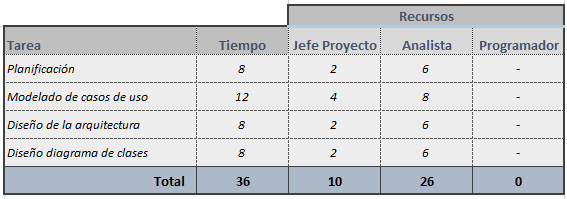
\includegraphics[
   keepaspectratio=true
]{./03_Met_Plan/02_Planificacion/img/PlanIter1.png}
\caption{Diagrama división tareas - iteración 1}
\end{figure}


\subsubsection*{Iteración 2: Base inicial proyecto}

\begin{figure}[H]
\vspace{-1cm}
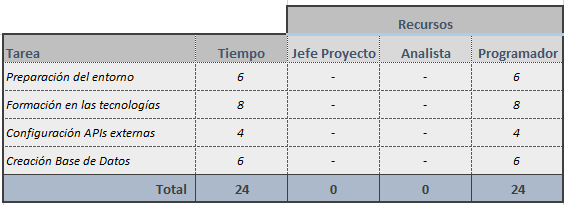
\includegraphics[
   keepaspectratio=true
]{./03_Met_Plan/02_Planificacion/img/PlanIter2.png}
\caption{Diagrama división tareas - iteración 2}
\end{figure}


\subsubsection*{Iteración 3: Usuarios}

\begin{figure}[H]
\vspace{-1cm}
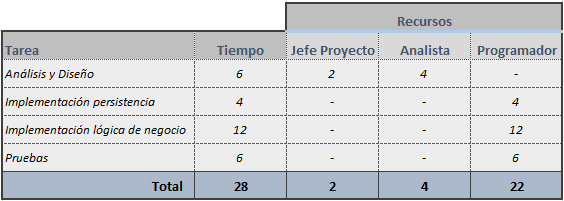
\includegraphics[
   keepaspectratio=true
]{./03_Met_Plan/02_Planificacion/img/PlanIter3.png}
\caption{Diagrama división tareas - iteración 3}
\end{figure}


\subsubsection*{Iteración 4: Rutas}

\begin{figure}[H]
\vspace{-1cm}
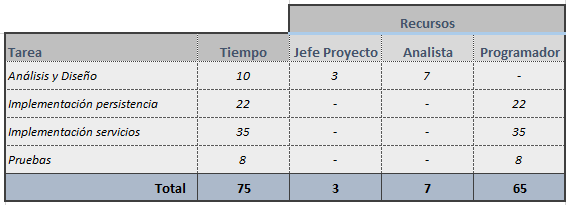
\includegraphics[
   keepaspectratio=true
]{./03_Met_Plan/02_Planificacion/img/PlanIter4.png}
\caption{Diagrama división tareas - iteración 4}
\end{figure}



\subsubsection*{Iteración 5: Eventos}

\begin{figure}[H]
\vspace{-1cm}
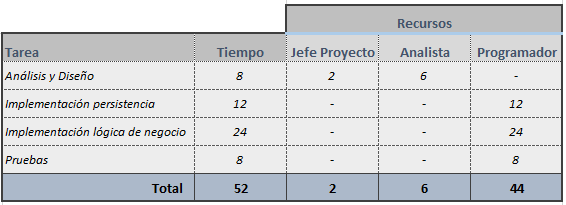
\includegraphics[
   keepaspectratio=true
]{./03_Met_Plan/02_Planificacion/img/PlanIter5.png}
\caption{Diagrama división tareas - iteración 5}
\end{figure}


\subsubsection*{Iteración 6: Servicios externos}

\begin{figure}[H]
\vspace{-1cm}
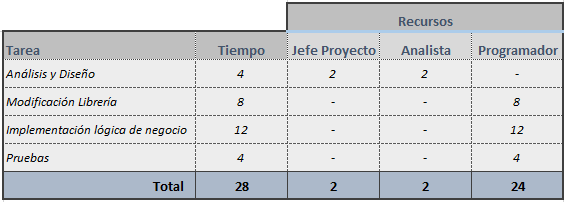
\includegraphics[
   keepaspectratio=true
]{./03_Met_Plan/02_Planificacion/img/PlanIter6.png}
\caption{Diagrama división tareas - iteración 6}
\end{figure}


\subsubsection*{Iteración 7: Lugares y categorías}

\begin{figure}[H]
\vspace{-1cm}
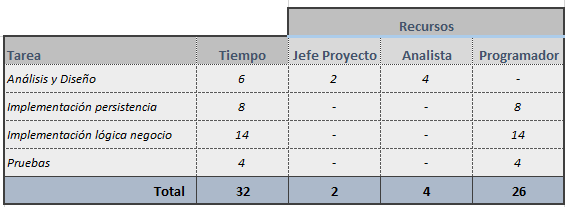
\includegraphics[
   keepaspectratio=true
]{./03_Met_Plan/02_Planificacion/img/PlanIter7.png}
\caption{Diagrama división tareas - iteración 7}
\end{figure}


\subsubsection*{Iteración 8: Capa servicios}

\begin{figure}[H]
\vspace{-1cm}
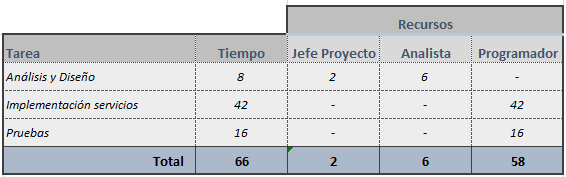
\includegraphics[
   keepaspectratio=true
]{./03_Met_Plan/02_Planificacion/img/PlanIter8.png}
\caption{Diagrama división tareas - iteración 8}
\end{figure}


\subsubsection*{Iteración 9: Autenticación y autorización}

\begin{figure}[H]
\vspace{-1cm}
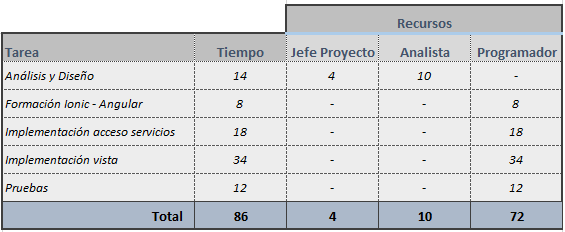
\includegraphics[
   keepaspectratio=true
]{./03_Met_Plan/02_Planificacion/img/PlanIter9.png}
\caption{Diagrama división tareas - iteración 9}
\end{figure}


\subsubsection*{Iteración 10: Cliente móvil}

\begin{figure}[H]
\vspace{-1cm}
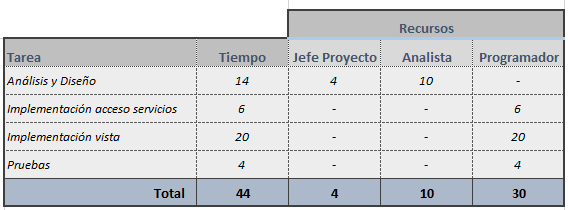
\includegraphics[
   keepaspectratio=true
]{./03_Met_Plan/02_Planificacion/img/PlanIter10.png}
\caption{Diagrama división tareas - iteración 10}
\end{figure}


\subsubsection*{Iteración 11: Cliente web}

\begin{figure}[H]
\vspace{-1cm}
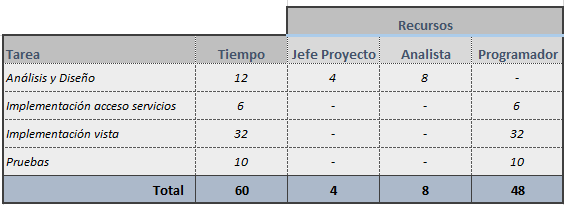
\includegraphics[
   keepaspectratio=true
]{./03_Met_Plan/02_Planificacion/img/PlanIter11.png}
\caption{Diagrama división tareas - iteración 11}
\end{figure}


\subsubsection*{Iteración 12: Panel de administración}

\begin{figure}[H]
\vspace{-1cm}
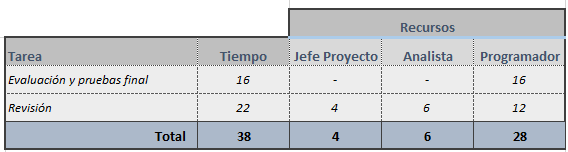
\includegraphics[
   keepaspectratio=true
]{./03_Met_Plan/02_Planificacion/img/PlanIter12.png}
\caption{Diagrama división tareas - iteración 12}
\end{figure}


\subsubsection*{Iteración 13: Cierre}

\begin{figure}[H]
\vspace{-1cm}
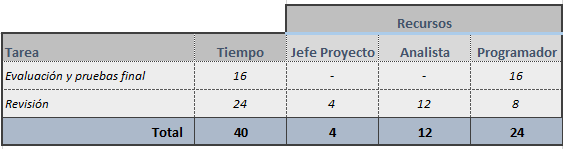
\includegraphics[
   keepaspectratio=true
]{./03_Met_Plan/02_Planificacion/img/PlanIter13.png}
\caption{Diagrama división tareas - iteración 13}
\end{figure}


\subsubsection*{Planificación global}

\begin{figure}[H]
\vspace{-0.5cm}
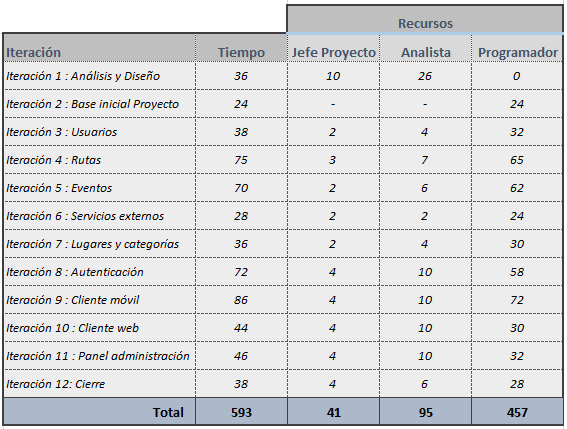
\includegraphics[
   keepaspectratio=true
]{./03_Met_Plan/02_Planificacion/img/PlanIterGlobal.png}
\caption{Diagrama división tareas - global}
\end{figure}

\newpage
\subsection{Planificación de las tareas}
En el siguiente diagrama se podrá observar la planificación total de proyecto así como la establecida en cada iteración.

\begin{figure}[H]
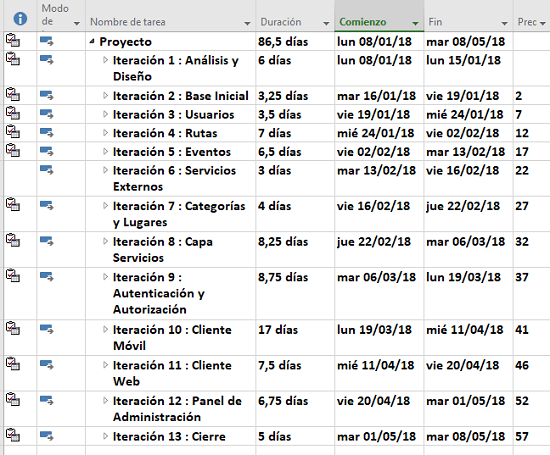
\includegraphics[
   keepaspectratio=true
]{./03_Met_Plan/02_Planificacion/img/gantt1.png}
\caption{Diagrama planificación - global}
\end{figure}

Observando el diagrama se puede observar la duración, la fecha de comienzo y de fin para el proyecto entero. Se muestra también la división y planificación del mismo, en las diferentes iteraciones definidas previamente. Para cada iteración, también se puede observar la planificación realizada.

En los siguiente diagramas se mostrará la planificación de las tareas para cada una de las iteraciones, indicando para cada una de ellas, el nombre, la fecha de inicio y fin, la duración, las tareas predecesoras y los recursos asignados encargados de realizar dicha tarea.


\begin{sidewaysfigure}
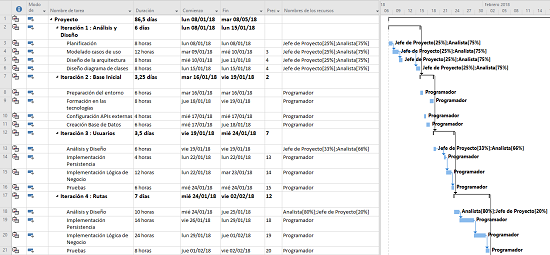
\includegraphics[
   keepaspectratio=true
]{./03_Met_Plan/02_Planificacion/img/gantt2.png}
\caption{Diagrama planificación - iteraciones 1-4}
\end{sidewaysfigure}

\begin{sidewaysfigure}
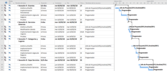
\includegraphics[
   keepaspectratio=true
]{./03_Met_Plan/02_Planificacion/img/gantt3.png}
\caption{Diagrama planificación - iteraciones 5-8}
\end{sidewaysfigure}

\begin{sidewaysfigure}
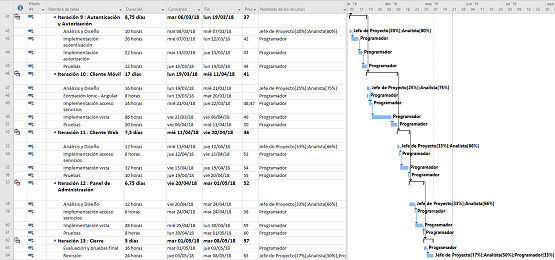
\includegraphics[
   keepaspectratio=true
]{./03_Met_Plan/02_Planificacion/img/gantt4.png}
\caption{Diagrama planificación - iteraciones 9-13}
\end{sidewaysfigure}




\section{Evaluación de costes}
\subsection{Recursos Humanos}
En la planificación del proyecto se han distinguido diferentes perfiles profesionales involucrados en la realización de las diferentes tareas. Conociendo el número total de horas trabajadas por cada recurso y su coste por hora, podemos calcular el coste total, de todos los recursos humanos, en el proyecto.

\begin{table}[H]
\centering
\begin{tabular}{|l|c|c|c|}
\hline
\textbf{Recurso} & \textbf{Coste/hora} & \textbf{Horas Trabajadas} & \textbf{Coste Total} \\ \hline
Jefe de Proyecto & 20 €/h & 38 & 760 €  \\ \hline
Analista & 18 €/h & 92 &  1.656 €  \\ \hline
Programador & 16 €/h & 492 & 7.872 €  \\ \hline
\textbf{Total} & & & \textbf{10.288 €} \\ \hline
\end{tabular}
\caption{Coste recursos humanos}
\end{table}


\subsection{Costes Hardware}
En cuanto al coste hardware se contabilizará únicamente los equipos utilizados para el desarrollo del proyecto. Una vez que la aplicación se lleve a la etapa de producción, se deberán contabilizar los gastos que supondrían mantener los servidores y equipos necesarios para su correcto funcionamiento.

En el desarrollo se ha empleado un ordenador personal del autor, con un coste aproximado de 1.300 euros.


\subsection{Costes Software}
Las principales herramientas software utilizadas en el desarrollo del proyecto son gratuitas. Únicamente, destacar el uso de una versión para estudiantes gratuita del software MagicDraw, y el uso de las versiones estándar de las APIs de Foursquare y Google que implican una serie de límites y restricciones, asumibles en el desarrollo y pruebas de la aplicación. 

Al igual que sucedía con los costes hardware, cuando la aplicación se encuentre en producción, será necesario asumir el coste de las versiones premium de las APIs mencionadas.


\subsection{Costes totales}
Como resultado de cada uno de las estimaciones de costes correspondientes a los recursos humanos, hardware y software; podemos estimar el coste total del desarrollo del proyecto.

\begin{table}[H]
\centering
\begin{tabular}{|l|c|c|c|}
\hline
\textbf{Recurso} & \textbf{Coste Total} \\ \hline
Recursos Humanos &  10.288 € \\ \hline
Hardware & 1.300 €  \\ \hline
Software & 0 €  \\ \hline
\textbf{Total} & \textbf{11.588 €} \\ \hline
\end{tabular}
\caption{Coste recursos totales}
\end{table}

Finalmente, se obtiene un coste total de 11.588 €.


\chapter[Análisis]{
  \label{chp:analisis}
  ANÁLISIS
}
\thispagestyle{numberingStyle}
\pagestyle{numberingStyle}

En este apartado se explicará, detalladamente, el análisis realizado.

\section{Análisis de requerimientos}

\subsection{Requerimientos funcionales}
A continuación se muestran los requerimientos funcionales del sistema, clasificados en distintas áreas.

\subsubsection*{Acceso a la aplicación}
\begin{itemize}
\setlength\itemsep{1pt}
\item El sistema ofrecerá la posibilidad de que un usuario se registre en la aplicación.
\item El sistema ofrecerá la posibilidad de que el usuario se identifique en el sistema. Los usuarios deben ingresar al sistema con  nombre de usuario y contraseña.
\end{itemize}

\subsubsection*{Aplicación Móvil}
\begin{itemize}
\setlength\itemsep{1pt}
\item El sistema ofrecerá la posibilidad de crear nuevas rutas.
\item El usuario podrá consultar las rutas, propias y de otros usuarios, según ciertos criterios de búsqueda.
\item El sistema permitirá a los usuarios autorizados eliminar las rutas propias que deseen.
\item El sistema permitirá a los usuarios autorizados a consultar los detalles de las rutas.
\item Para las rutas, el sistema permitirá:
	\begin{itemize}
	\item Establecer las fechas de inicio y fin.
	\item Consultar, asignar y desasignar a la ruta, los eventos disponibles en esas fechas.
	\item Consultar el itinerario por días.
	\item Modificar la hora de comienzo establecida para cada día.
	\item Consultar, añadir y eliminar lugares de interés a cada día de la ruta.
	\item Editar el modo de viaje a realizar entre diferentes lugares.
	\item Mostrar el itinerario, por días y en total, en el mapa.
	\item Habilitar y deshabilitar el sistema de geolocalización para conocer la ruta hecha en tiempo real.
	\item Consultar y comparar, el itinerario definido con el obtenido a tiempo real.
	\item Editar los permisos de la ruta.
	\end{itemize}
\end{itemize}

\subsubsection*{Aplicación Web}
\begin{itemize}
\setlength\itemsep{1pt}
\item El usuario podrá consultar las rutas existentes, propias y de otros usuarios, según ciertos criterios de búsqueda.
\item El sistema permitirá a los usuarios autorizados a consultar los detalles de las rutas.
\item El sistema permitirá a los usuarios autorizados marcar las rutas propias como privadas, con el fin de no compartirlas con los demás usuarios.
\item El sistema solo ofrecerá la posibilidad de consulta sobre los detalles de una ruta, permitiendo ver el itinerario, si tiene datos en tiempo real guardados, etc...
\item El sistema permitirá a los usuarios autorizados eliminar las rutas propias que deseen.
\end{itemize}

\subsubsection*{Administración Web}
\begin{itemize}
\setlength\itemsep{1pt}
\item El sistema solo permitirá acceso a usuarios con permisos de administración.
\item El sistema permitirá a los usuarios con dichos permisos, dar de alto nuevos usuarios.
\item El sistema permitirá las altas, bajas, modificaciones y consultas de las entidades del sistema.
	\begin{itemize}
	\item El sistema ofrecerá la posibilidad de crear, eliminar, modificar y consultar datos de usuarios.
	\item El sistema ofrecerá la posibilidad de crear, eliminar, modificar y consultar datos de rutas.
	\item El sistema ofrecerá la posibilidad de crear, eliminar, modificar y consultar datos de lugares.
	\item El sistema ofrecerá la posibilidad de crear, eliminar, modificar y consultar datos de categorías.
	\item El sistema ofrecerá la posibilidad de crear, eliminar, modificar y consultar datos de eventos.
	\end{itemize}

\end{itemize}

\subsubsection*{Seguridad}
\begin{itemize}
\setlength\itemsep{1pt}
\item El sistema ofrecerá la posibilidad de que el usuario modifique sus datos de acceso al sistema.
\item El sistema solo permitirá acciones correctamente autenticadas, exceptuando las de acceso a la aplicación.
\item Los usuarios de la aplicación solo podrán modificar los datos a los que el usuario esté autorizado. Un usuario no podrá modificar la información de los recursos de los que no es propietario.
\item Los intercambios de datos que realice el sistema a través de internet, serán mediante el uso del protocolo encriptado https.
\end{itemize}


\subsection{Requerimientos no funcionales}
\subsubsection*{Rendimiento}
\subsubsection*{Disponibilidad}
\subsubsection*{Estabilidad}
\subsubsection*{Escalabilidad}




\section{Modelo de casos de uso}

\subsection{Actores del sistema}

\subsection{Diagrama de casos de uso}
Tras conocer los requerimientos funcionales del sistema, se ha optado por la elaboración de dos diagramas de casos de uso. El primero con las necesidades del cliente móvil y el segundo con las de la parte web.


\begin{figure}[t!]
Para el cliente móvil, presentamos el siguiente diagrama.
\\

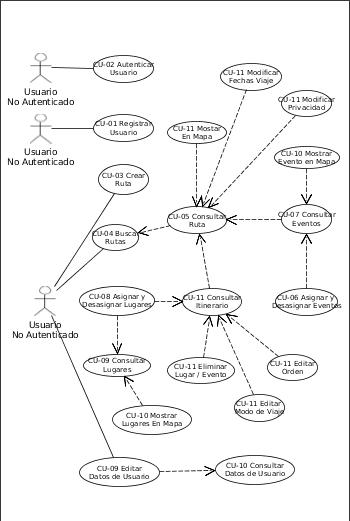
\includegraphics[
   keepaspectratio=true
]{usecase-app-movil.jpg}
\caption{Diagrama Casos de Uso Aplicación Móvil.}
\end{figure}









\newpage
\subsection{Especificación casos de uso}


\newpage
\subsubsection*{Autenticar Usuario}
\begin{longtable}{| p{4cm} | p{10cm} |}
\endfirsthead
\multicolumn{2}{c}{\textit{Continúa de la página anterior}}\\[12pt]
\hline
\endhead
\hline
\multicolumn{2}{c}{\textit{Continúa en la siguiente página}} \\
\endfoot
\hline
\caption{Caso de Uso: Autenticar Usuario}\label{fig:1}\\
\endlastfoot


\hline
\multicolumn{2}{|c|}{\textbf{CU$<$01$>$ Autenticar Usuario}} \\

\hline
\textbf{Descripción} &
El usuario se identifica introduciendo las credenciales de acceso en el sistema \\

\hline
\textbf{Actores} &
Usuario\newline
Administrador\newline
Moderador\\

\hline
\textbf{Precondiciones} &
N/A\\

\hline
\textbf{Secuencia Normal} &\mbox{}\par\vspace{-\baselineskip}
\begin{enumerate}[leftmargin=0.7cm, topsep=0.1cm]
\item El usuario introduce sus credenciales en la ventana de login. 
\item El usuario pulsa el botón de \textit{Acceder}.
\item El sistema valida las credenciales.
\item El usuario accede a la aplicación.
\end{enumerate}\\

\hline
\textbf{Excepciones} &\mbox{}\par\vspace{-\baselineskip}
\begin{enumerate}[leftmargin=0.9cm, topsep=0.1cm]
\item[3a.] Los datos introducidos no son correctos.
	\begin{itemize}
	\item[1.] El usuario vuelve a introducir las credenciales.
	\end{itemize}

\end{enumerate}\\

\hline
\textbf{Postcondiciones} & 
El usuario queda autenticado en el sistema\\
\hline
\end{longtable}




\newpage
\subsubsection*{Registrar Usuario}
\begin{longtable}{| p{4cm} | p{10cm} |}
\endfirsthead
\multicolumn{2}{c}{\textit{Continúa de la página anterior}}\\[12pt]
\hline
\endhead
\hline
\multicolumn{2}{c}{\textit{Continúa en la siguiente página}} \\
\endfoot
\hline
\caption{Caso de Uso: Registrar Usuario}\label{fig:1}\\
\endlastfoot


\hline
\multicolumn{2}{|c|}{\textbf{CU$<$02$>$ Registrar Usuario}} \\

\hline
\textbf{Descripción} &
El usuario introduce los datos para darse de alta en la aplicación. \\

\hline
\textbf{Actores} &
Usuario\\


\hline
\textbf{Precondiciones} &
N/A\\

\hline
\textbf{Secuencia Normal} &\mbox{}\par\vspace{-\baselineskip}
\begin{enumerate}[leftmargin=0.7cm, topsep=0.1cm]
\item El usuario selecciona la opción de registrarse.
\item El sistema muestra un formulario indicando los campos necesarios para realizar el registro.
\item El usuario rellena los campos y pulsa el botón de \textit{Registrarse}.
\item El sistema valida los datos introducidos por el usuario.
\item El usuario accede a la aplicación.
\end{enumerate}\\

\hline
\textbf{Excepciones} &\mbox{}\par\vspace{-\baselineskip}
\begin{enumerate}[leftmargin=0.9cm, topsep=0.1cm]
\item[3a.] El usuario pulsa el botón de \textit{Cancelar}.
	\begin{itemize}
	\item[1.] El sistema cancela el registro y redirige al usuario a la pantalla de login.
	\item[2.] Implementa CU-$<$01$>$ Autenticar Usuario
	\end{itemize}
\item[3a.] Los datos introducidos por el usuario no son válidos.
	\begin{itemize}
	\item[1.] El sistema muestra un mensaje de error e invita al usuario a volver a introducir los datos. (Regreso al paso 2)
	\end{itemize}

\end{enumerate}\\

\hline
\textbf{Postcondiciones} & 
El usuario queda registrado y autenticado en el sistema\\
\hline
\end{longtable}

\chapter[Dise\~no]{
  \label{chp:diseno}
  DISE\~NO
}
\thispagestyle{numberingStyle}
\pagestyle{numberingStyle}


\section{Arquitectura del sistema}
La arquitectura empleada en nuestro sistema será una arquitectura en capas, una de las técnicas de diseño más usadas en las ciencias de la computación. La arquitectura basada en capas es una especialización de la arquitectura cliente-servidor donde la carga de trabajo se divide en diferentes capas con un reparto claro de las funciones.

En esta arquitectura, una capa inferior proporciona un servicio a otra copa superior. El servicio ofrecido se define mediante un contrato de servicio. De esta forma, se consigue independizar el software de ambas capas y los cambios de implementación en una de ellas no tienen repercusión sobre las demás.

Partiendo que la aplicación será accesible desde dispositivo móvil y navegador web, se presentará una solución al diseño basada en dos alternativas de la arquitectura basada en capas: la arquitectura en 3 capas y la arquitectura en 4 capas.


\subsection{Arquitectura en 3 capas físicas}
En este sistema de arquitectura, se diferencian tres capas físicas que cumplen funciones diferentes.
\\
\\ 

\begin{figure}[!h]

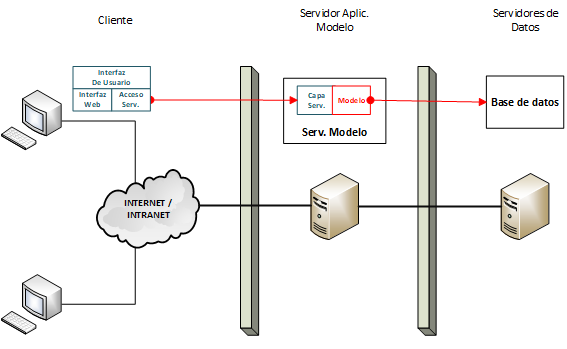
\includegraphics[
   keepaspectratio=true
]{./05_Diseno/arq3capas.png}
\caption{Diagrama arquitectura en tres capas}
\end{figure}

\begin{itemize}
	\item \textbf{Capa Física - Servidor de Datos: } Es la capa encargada de gestionar el almacenamiento de los datos.
	\item \textbf{Capa Física - Servidor Aplicación Modelo:} Formada por las siguientes capas lógicas.
	\begin{itemize}
		\item \textbf{Capa Modelo:} Es la encargada implementar las funcionalidades de la aplicación y mantener la comunicación con el servidor de datos realizando las acciones relacionadas con el acceso a los datos. Comúnmente, se subdivide en dos, la capa de acceso a datos, para la conexión con el servidor de datos, y la capa lógica de negocio, para la implementación de los casos de uso.
		\item \textbf{Capa Servicios: } Sirve de enlace entre la interfaz de usuario y la capa modelo. 
	\end{itemize}		
	\item \textbf{Capa Física - Cliente: } Divida en las siguientes capas lógicas.
	\begin{itemize}
		\item \textbf{Capa de Acceso al Servicio: } Capa encargada de acceder e invocar a los métodos de la capa de servicios del modelo.
		\item \textbf{Capa Interfaz de Usuario: } Interfaz gráfica final que se instala en las máquinas cliente y dispositivos finales.
	\end{itemize}
\end{itemize}



\subsection{Arquitectura en 4 capas físicas}
En esta alternativa, se añade una capa intermedia entre el cliente y el modelo que actúe de servidor de aplicaciones y que proporciones la interfaz web para clientes que accedan desde navegador web.

\begin{figure}[!h]

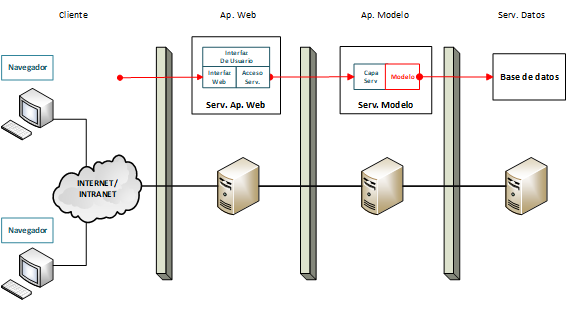
\includegraphics[
   keepaspectratio=true
]{./05_Diseno/arq4capas.png}
\caption{Diagrama arquitectura en cuatro capas}
\end{figure}

Un navegador, para acceder a la aplicación, necesitará de un servidor de aplicaciones que le proporcione la interfaz web. Incorporar esta interfaz dentro del servidor de aplicaciones visto en la arquitectura anterior haría que este y el modelo estén fuertemente acoplados, impidiendo que puedan ser construidos con tecnologías diferentes.

Por ello, con esta arquitectura se pretende hacer ese desacople consiguiendo que múltiples aplicaciones puedan invocar al modelo, independientemente de que sean con interfaz gráfica o mediante navegador, sin necesidad de replicar el código del modelo en cada aplicación.

En consecuencia, analizados los requisitos del sistema y conociendo las necesidades del mismo, se diseñará un sistema basado en una arquitectura de cuatro capas desde el punto de vista de un cliente web, y de tres capas, desde el punto del cliente móvil.


\subsection{Arquitectura completa del sistema}
A continuación, se presenta el diseño completo que se elaborará en la aplicación.

\begin{figure}[!h]

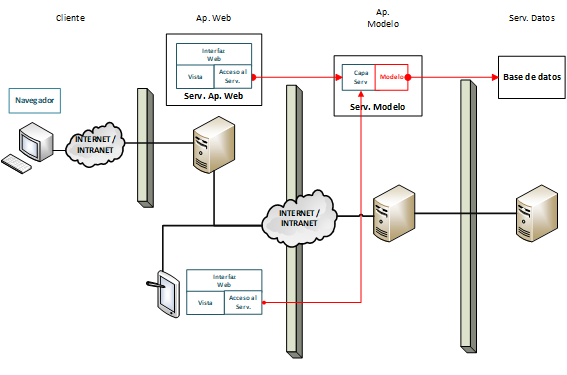
\includegraphics[
   keepaspectratio=true
]{./05_Diseno/arqsistema.png}
\caption{Diagrama arquitectura completa del sistema}
\end{figure}

Como se puede observar en el diagrama, el sistema sigue una arquitectura en cuatro capas.

Al tener la aplicación modelo desacoplada de la aplicación web, la capa de servicios debe servir de enlace entre la capa modelo y la interfaz de usuario. Ese enlace lo ofrece mediante unos servicios REST, que exponen a la capa superior, las funcionalidades implementadas en la capa modelo.

Por su parte, en las aplicaciones cliente, la interfaz web del servidor de aplicaciones y la interfaz del cliente móvil, siguen el patrón de arquitectura Modelo-Vista-Controlador (MVC) y Modelo-Vista-VistaModelo (MVVM), respectivamente. En ellas, el modelo no se encuentra implementado en la propia aplicación, sino que se accede, a través de la capa de acceso a los servicios, que son ofrecidos por el modelo. De esta forma, ambas aplicaciones finales, invocan al modelo sin necesidad de tenerlo replicado.



\section{Diseño físico de los datos}
\subsection{Modelo Entidad-Relación}
\begin{figure}[H]
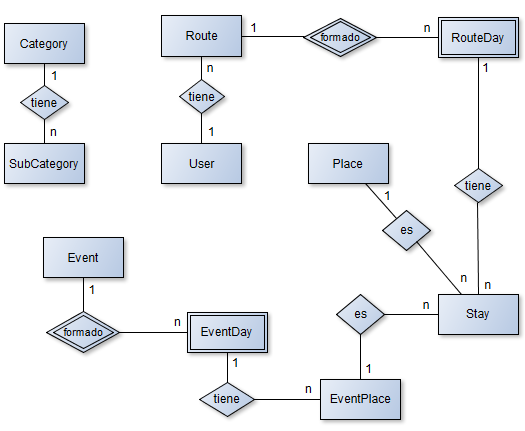
\includegraphics[
   keepaspectratio=true
]{./05_Diseno/ER.png}
\caption{Diagrama Entidad-Relación}
\end{figure}

En el apéndice se incluye un diagrama Entidad-Relación completo, incluyendo entidades y atributos.


\section{Capa Modelo}
Esta capa es la encargada de implementar la lógica de negocio de la aplicación, lo que implica el manejo de las entidades persistentes y el acceso a los datos. Como podemos observar en la Figura 6.4, y debido a la arquitectura establecida, el modelo estará compuesto por la capa de acceso a datos y la capa de lógica de negocio.

\begin{figure}[H]
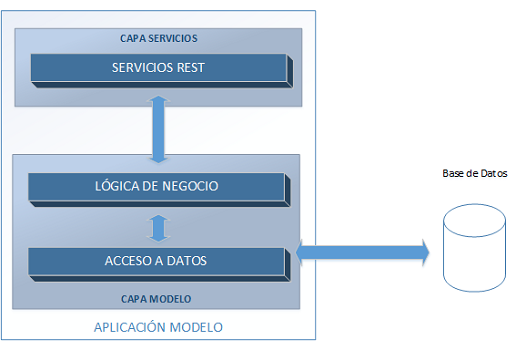
\includegraphics[
   keepaspectratio=true
]{./05_Diseno/disenomodelo.png}
\caption{Diagrama diseño modelo}
\end{figure}


\subsection{Diseño módulo acceso a datos}
En la capa de acceso a datos se definirán el conjunto de entidades persistentes que manejará la aplicación y se empleará el patrón de diseño Data-Access-Object (DAO) para abstraer la persistencia de las entidades así como la fuente de datos empleada.

Por cada entidad persistente existirá un DAO encargado de gestionar la comunicación con la fuente de datos empleada.

\newpage
\subsubsection*{Diagrama clases persistentes}
\begin{figure}[H]
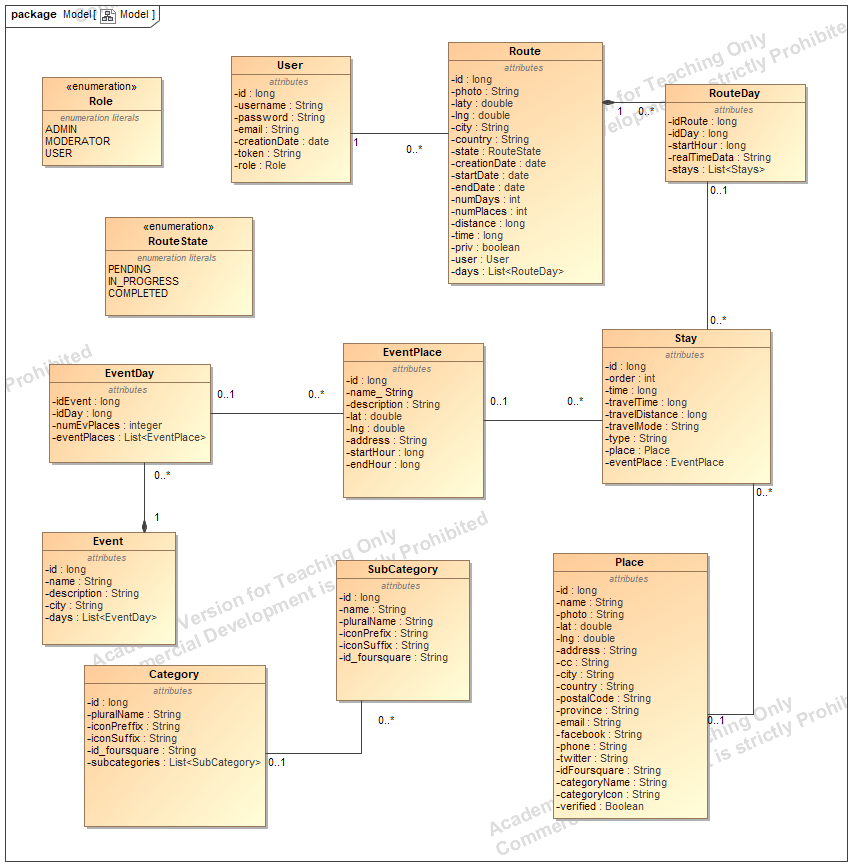
\includegraphics[
   keepaspectratio=true
]{./05_Diseno/disenoclases.png}
\caption{Diagrama clases persistentes}
\end{figure}

En el diagrama se muestran las clases persistentes que manejará la aplicación. A continuación, se detallará brevemente, el significado y funcionalidad de cada una:

\begin{itemize}
	\item \textbf{User: } Es la clase encargada de representar la información de los usuarios registrados en la aplicación.
	\item \textbf{Role: } Enumerado con los roles disponibles para un usuario: \textit{ADMIN, MODERATOR y USER}.
	\item \textbf{Route: } Clase encargada de guardar la información sobre las rutas creadas por los usuarios. Las rutas están compuestas por \textit{RouteDays}.
	\item \textbf{RouteDay: } Clase con una relación fuerte de composición con la clase \textit{Route}. Su tiempo de vida está condicionada por la vida de la clase que la incluye. Mantiene la información para cada uno de los días que componen la duración de una ruta.
	\item \textbf{RouteState: } Enumerado con los diferentes estados por los que pasa una ruta en el tiempo: \textit{PENDING, IN\_PROGRESS y COMPLETED}.
	\item \textbf{Stay: } Entidad con la funcionalidad de almacenar las visitas que decida hacer un usuario en un día de una ruta determinada. La visita, puede ser a lugares obtenidos de la fuente externa (Foursquare) o a eventos gestionados por la propia aplicación.
	\item \textbf{Place: } Entidad que registra y almacena los detalles sobre los lugares extraídos de la fuente externa.
	\item \textbf{Event: } Es la clase encargada de representar los eventos dados de alta en el sistema. Los eventos están compuestos por \textit{EventDays}.
	\item \textbf{EventDay: } Clase con una relación fuerte de composición con la clase \textit{Event}. Su tiempo de vida está condicionada por la vida de la clase que la incluye. Mantiene la información para cada uno de los días que componen al evento.
	\item \textbf{EventPlace: } Es la clase donde se maneja toda la información sobre las distintas ubicaciones y actividades que incluye un día determinado del evento.
	\item \textbf{Category: } Clase que almacena la información relevante a las categorías sobre las que se filtran los lugares obtenidos de Foursquare.
	\item \textbf{SubCategory: } Establece una jerarquía con la clase anterior. Almacena las categorías que son un subtipo de una categoría determinada.
\end{itemize}


\subsubsection*{Patrón de diseño DAO}
Este patrón de diseño intenta desacoplar el acceso a los datos de su almacenamiento subyacente. Los datos persistentes, actualmente, dependen en gran medida del tipo de base de datos utilizada: base de datos relacional, base de datos orientada a objetos, archivos planos... siendo las bases de datos relacionales las más utilizadas. 

Partiendo de que los accesos a diferentes tipos de bases de datos se realizan de manera muy diferente, utilizar este patrón en lugar de acceder directamente a la fuente de datos, nos permite pasar de un tipo de fuente de datos a otro diferente sin tener que realizar modificaciones en la lógica de negocio.


\begin{figure}[H]
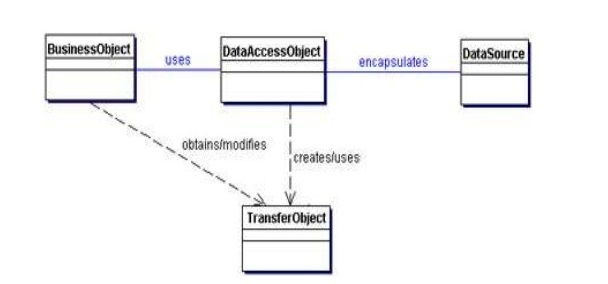
\includegraphics[
   keepaspectratio=true
]{./05_Diseno/patrondao.jpg}
\caption{Diagrama patrón DAO}
\end{figure}

En la Figura 6.6 se muestra un pequeño diagrama con los elementos participantes en este patrón de diseño.

\begin{itemize}
	\item \textbf{Business Object: } Representa la clase con la lógica de negocio. Es la responsable de saber qué y cómo modificar el contenido de los datos pero no cómo almacenarlo.
	\item \textbf{Data Access Object: } Se encarga de ocultar la fuente de datos real de manera que el objeto con la lógica de negocio (Business Object) se comunica con este en vez de hacerlo directamente con el objeto de acceso a los datos.
	\item \textbf{DataSource: } Es la clase encargada de obtener las conexiones a la base de datos.
	\item \textbf{Transfer Object: } Es el objeto que se utiliza para transferir el contenido de los datos reales, del \textit{Data Access Object} al objeto de negocio \textit{Business Object}. Representa los datos almacenados en la base de datos.
\end{itemize}


\subsubsection*{Diseño de los DAOs}
\begin{figure}[H]
\centering
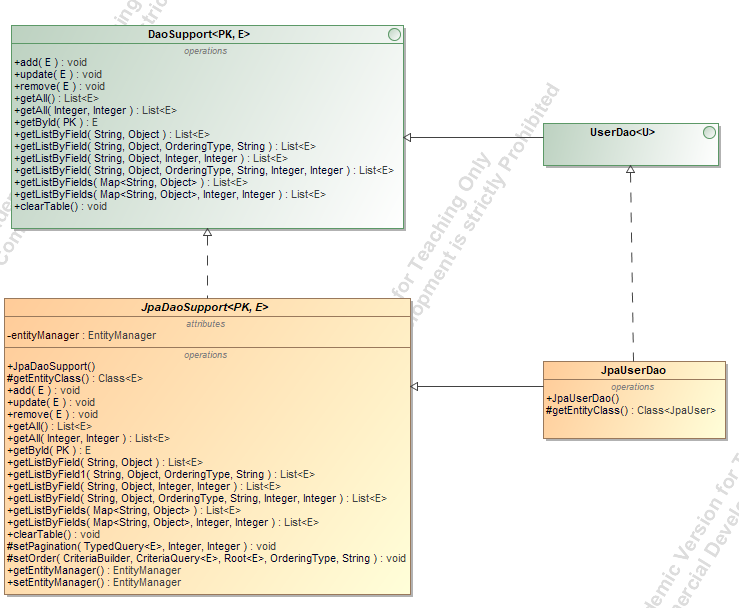
\includegraphics[
   keepaspectratio=true
]{./05_Diseno/userdao.png}
\caption{Diagrama ejemplo UserDao}
\end{figure}

En la figura 6.8 se muestra un esquema en el que se define e implementa un DAO genérico que proporciona las principales operaciones de acceso a datos, permitiendo que las definiciones de DAOs, que extiendan a este DAO genérico, tengan las operaciones básicas sin necesidad de definirlas ni implementarlas. Del mismo modo, en los DAOs que extiendan el DAO genérico, también se podrán definir e implementar funcionalidades específicas para cada uno de ellos. Este ejemplo, del DAO de la entidad \textit{User}, se compone de:

\begin{itemize}
	\item \textbf{DaoSupport: } Interfaz que define una serie de métodos y operaciones sobre los datos.
	\item \textbf{JpaDaoSupport: } Clase genérica que implementa las funciones de la interfaz anterior.
	\item \textbf{UserDao: } Definición del DAO específico para la entidad \textit{User}. Extiende las funcionalidades de la interfaz \textit{DaoSupport} y en este caso, no incluye ningún más.
	\item \textbf{JpaUserDao: } Implementación de \textit{UserDao} que extiende la implementación de las funciones de la clase genérica. 
\end{itemize}

Este esquema se repite con todas las entidades, exceptuando aquellas que necesitan de una relación con otra entidad para existir. Por ejemplo, la entidad \textit{RouteDay} necesita de \textit{Route} para existir, por lo que su identificador es dependiente de la otra entidad. Para este tipo de entidades, que no pueden seguir las definiciones del DAO genérico explicado anteriormente por estar diseñado únicamente para entidades formadas por identificadores de un único atributo, se presenta una solución particular para cada entidad, donde cada DAO define e implementa sus funcionalidades necesarias. 

Este diseño y el de todos los DAOs se puede observar en el Apéndice .... (Añadir a apendice)


\newpage
\subsection{Diseño módulo lógica de negocio}
En este módulo o subcapa es donde se implementan y desarrollan los casos de uso previamente especificados.

En el diseño de los servicios ofrecidos se utilizará el patrón de diseño Fachada. Con este patrón, se crearán una serie de servicios que agruparán y gestionarán un conjunto determinado de entidades y componentes ofrecidos por la capa de acceso a datos. Estos servicios ofrecerán una serie de funcionalidades abstrayendo la complejidad de implementación y de dependencia con demás componentes.

\subsubsection*{Patrón Fachada}
El propósito del patrón de diseño Fachada es proporcionar una interfaz unificada para un conjunto de interfaces en un subsistema. Se define una interfaz de nivel superior lo que permite hacer el subsistema más fácil de utilizar.

\begin{figure}[H]
\centering
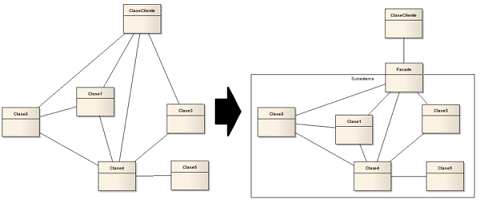
\includegraphics[
   keepaspectratio=true
]{./05_Diseno/patronfacade.png}
\caption{Ejemplo patrón de diseño Fachada}
\end{figure}

Estructurar un sistema en subsistemas ayuda a reducir la complejidad. Uno de los objetivos más comunes de diseño es minimizar la comunicación y las dependencias entre los subsistemas. Esto se puede lograr haciendo uso de este patrón.

Como podemos observar en la Figura 6.7, utilizando el patrón fachada se proporciona una interfaz única de acceso que se encargar de gestionar las comunicaciones y dependencias necesarias con otros módulos o subsistemas para realizar sus funcionalidades. Permite abstraer al cliente de cómo se gestionan las comunicaciones con los diferentes módulos.


\subsubsection*{Diseño de los servicios}
\begin{figure}[H]
\centering
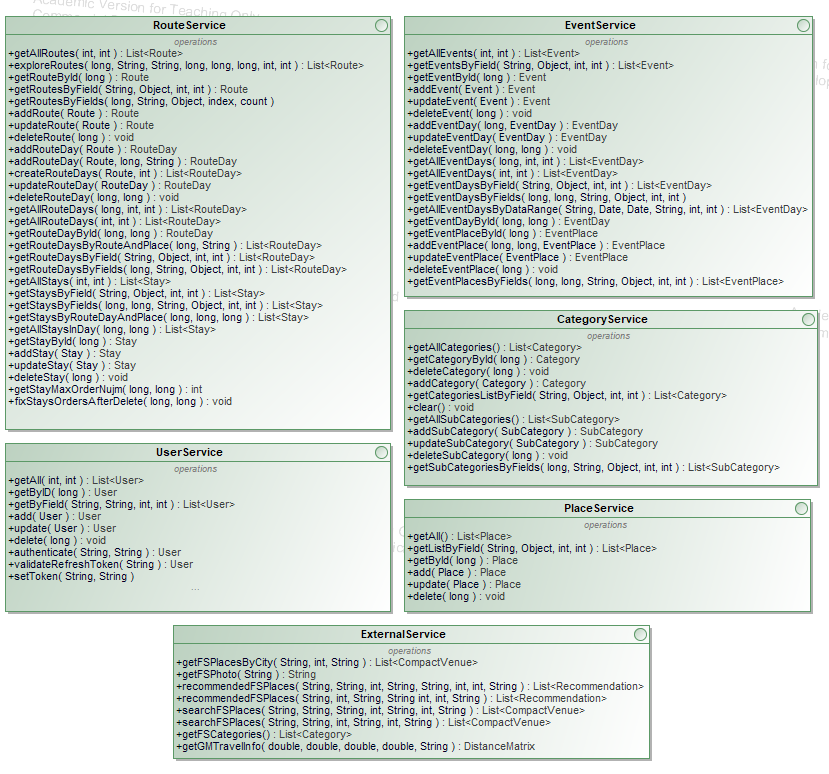
\includegraphics[
   keepaspectratio=true
]{./05_Diseno/disenoservicios.png}
\caption{Diagrama diseño servicios}
\end{figure}

En la Figura 6.8 podemos ver el diseño de los servicios que implementarán las funcionalidades de la aplicación. Se detallan brevemente a continuación:

\begin{itemize}
	\item \textbf{RouteService: } Servicio encargado de implementar los casos de uso o funcionalidades referentes a las rutas. Gestionan tanto las propias rutas como su composición por días y las visitas incluidas en cada día.
	\item \textbf{EventService: } Este servicio es el encargado de la gestión de los eventos en la aplicación. Al igual que con el anterior servicio, este incluye las funcionalidades para gestionar la composición por días y los lugares o ubicaciones específicas que existan dentro de un mismo evento.
	\item \textbf{UserService: } Ofrece los casos de uso referente a la entidad usuarios. Incluye desde el manejo de los datos sobre los usuarios hasta las funcionalidades de autenticación.
	\item \textbf{CategoryService: } Es el servicio encargado de administrar las categorías.
	\item \textbf{PlaceService: } Presenta las funcionalidades necesarias para gestionar los lugares que se registran en la aplicación.
	\item \textbf{ExternalService: } Es el servicio encargado de ofrecer las funciones que requieren de una comunicación con fuentes de datos externos. En este caso, se proporcionará una implementación que hará uso de las APIs de Foursquare y de Google Maps.
\end{itemize}

\subsubsection*{Diagrama ejemplo patrón fachada}
\begin{figure}[H]
\centering
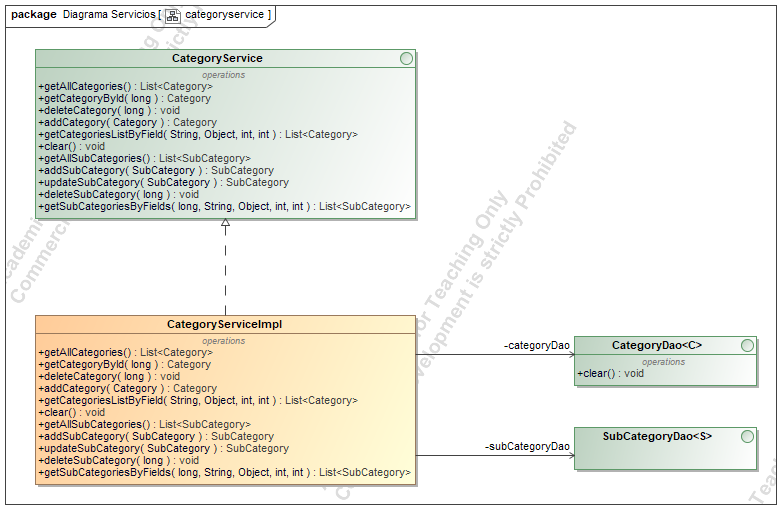
\includegraphics[
   keepaspectratio=true
]{./05_Diseno/categoryservice.png}
\caption{Diagrama ejemplo \textit{CategoryService}}
\end{figure}

En la figura 6.11, podemos ver el ejemplo de un servicio concreto, en este caso \textit{CategoryService}. En este ejemplo, podemos observar la definición del servicio a través de la interfaz \textit{CategoryService} y donde su implementación es la encargada de gestionar las comunicaciones con los diferentes módulo y subsistemas, en este caso, con los DAOs de las entidades \textit{Category} y \textit{SubCategory}.



\section{Capa servicios}
La capa de servicios ofrecerá las funcionalidades de la capa modelo a través de recursos accesibles por la red, mediante peticiones HTTP. Se proporcionará una implementación de la capa de servicios siguiendo el  estilo arquitectónico Representational State Transfer (REST) mediante el uso del API de programación JAX-RS.

Se utilizará el patrón de diseño Data Transfer Object (DTO).

\subsubsection*{Patrón de diseño DTO}
Es un patrón de diseño que se utiliza para transferir varios atributos entre un cliente y un servidor, o viceversa. De esta forma se consigue encapsular los objetos de negocio de manera que, cuando un cliente solicita al servidor determinada información, este construye un objeto de transferencia que rellena con los atributos del objeto de negocio y se lo envía finalmente al cliente.

Generalmente, este patrón de diseño está compuesto por las siguientes clases:

\begin{itemize}
	\item \textbf{Objeto de transferencia: } Clase POJO únicamente compuesta por atributos y métodos de lectura y escritura.
	\item \textbf{Clase de negocio: } Clase encargada de implementar las funcionalidades de la aplicación. Envía o recibe la clase \textit{Objeto de transferencia} por parte del cliente, que modifica utilizando los datos de la base de datos.
\end{itemize}


\subsubsection*{Diagrama módulo REST}
A continuación se mostrará un diagrama de ejemplo, con las clases involucradas en la gestión de los casos de uso de usuarios.

\begin{figure}[H]
\centering
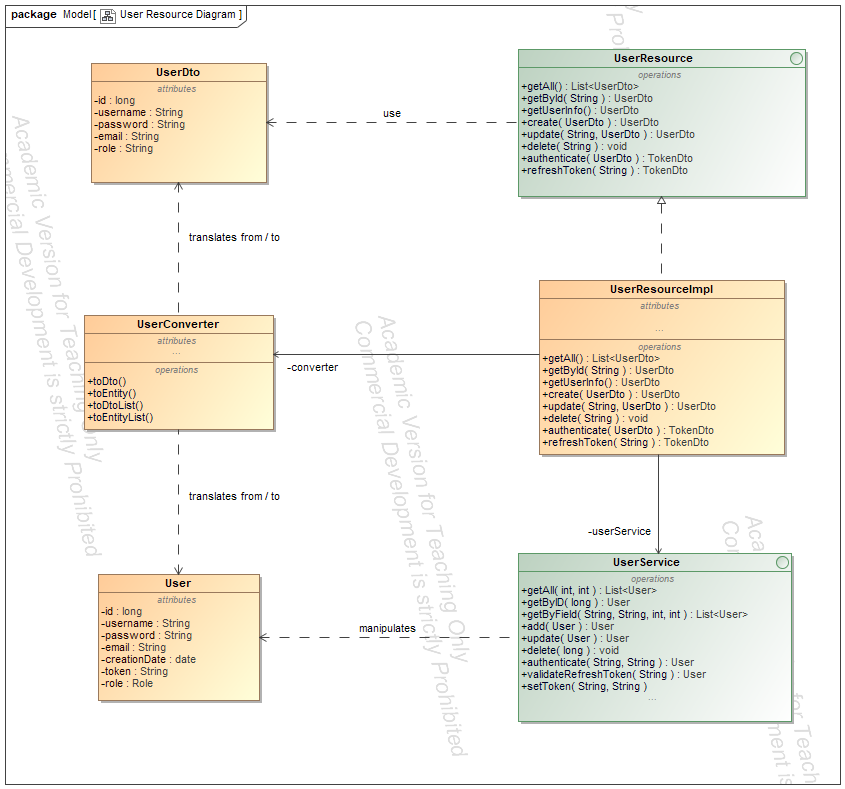
\includegraphics[
   keepaspectratio=true
]{./05_Diseno/disenorest.png}
\caption{Diagrama ejemplo servicios usuario}
\end{figure}


\begin{itemize}
	\item \textbf{UserDto: } Es el objeto de transferencia.
	\item \textbf{User: } Objeto de negocio para la entidad usuario.
	\item \textbf{UserResource: } Interfaz que expone ciertas funcionalidades a través de un recurso web. En este ejemplo, se define la implementación \textit{UserResourceImpl}, encargada de implementar las funciones establecidas en la interfaz. Los datos e información manejada se hace a través del objeto de transferencia.
	\item \textbf{UserService: } Servicio ofrecido por la capa modelo que gestiona los casos de uso y funcionalidades referentes a usuarios. Manipula el objeto de negocio \textit{User} y sus funcionalidades son invocadas por parte de \textit{UserResouceImpl}.
	\item \textbf{UserConverter: } Clase de utilidad que permite a la implementación del recurso \textit{UserResource} transformar el objeto de negocio en un objeto de transferencia, y viceversa.

\end{itemize}

El resto de servicios definidos en la aplicación seguirán una estructura similar. Se ofrecerán recursos web accesibles mediante HTTP que permitirán la invocación remota de la lógica de negocio de la aplicación.


\section{Capa Interfaz}
La capa interfaz, también conocida como capa cliente o capa de presentación, es la encargada de separar la interacción del usuario respecto a la lógica de negocio. Esta capa simplemente presenta la información al usuario y recibe las peticiones que debe comunicar a la capa modelo.

En nuestro sistema, existen dos presentaciones de la aplicación completamente diferentes e independientes: una aplicación web accesible desde navegador web y una aplicación para dispositivos móviles.

\subsection{Aplicación web}
La aplicación web se ejecutará en un servidor de aplicaciones que recibirá y gestionará todas las peticiones del cliente. Será la encargada de generar la vista web de la aplicación así como comunicarse con la capa modelo, accediendo a la capa de servicios del modelo.

Seguirá el patrón de arquitectura Modelo-Vista-Controlador (MVC).

\subsubsection*{Patrón Modelo-Vista-Controlador}
MVC es un patrón de arquitectura de software que separa los datos y la lógica de negocio, de su representación. Está formado por tres componentes distintos: modelo, vista y controlador.

El modelo es la información de la aplicación y el que proviene de la lógica de negocio. La vista, por su parte, es la representación en pantalla mientras que el controlador es el encargado de mantener la comunicación con el modelo y definir la forma en que la interfaz reacciona a las peticiones del usuario. Antes del patrón MVC, los diseños de interfaz de usuario tendían a agrupar estos objetos. Con este patrón se consigue desacoplar vistas y modelos estableciendo un protocolo de `suscripción-notificación' entre ellos.

\subsubsection*{Diagrama MVC aplicación web}
A continuación se mostrará un diagrama donde se verán los componentes MVC anteriormente comentados en el sistema de nuestra aplicación web.

\begin{figure}[H]
\centering
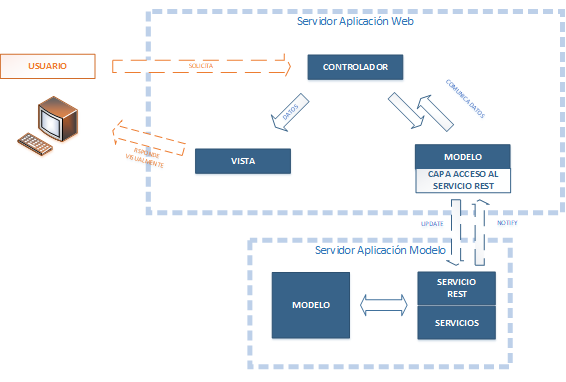
\includegraphics[
   keepaspectratio=true
]{./05_Diseno/mvccapaweb.png}
\caption{Diagrama MVC aplicación web}
\end{figure}

El controlador recibirá las solicitudes del usuario y obtendrá los datos del modelo a través del servicio REST especificado. Con estos datos, el controlador creará la vista correspondiente, que será entregada al usuario.


\subsubsection*{Diseño capa acceso al servicio}
En la siguiente figura se mostrará el diseño que permitirá invocar a la capa de servicios del modelo.
\begin{figure}[H]
\centering
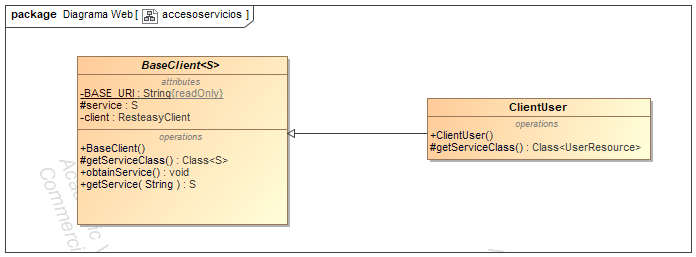
\includegraphics[
   keepaspectratio=true
]{./05_Diseno/accesoservicios.png}
\caption{Diagrama ejemplo acceso a servicios cliente web}
\end{figure}

En este diagrama se definen dos clases: \textit{BaseClient} y \textit{ClientRoute}. La primera es la encargada de crear un cliente que permita construir peticiones HTTP que se usarán para invocar los métodos ofrecidos en la capa de servicios.

Por su parte, la clase \textit{ClientRoute}, modifica el comportamiento de la clase anterior indicando sobre qué recurso tiene que elaborar las peticiones HTTP. En este ejemplo, se utiliza el recurso \textit{RouteResource} de la capa de servicios. Análogamente, se crean las diferentes clases clientes, para acceder a los diferentes recursos creados en la capa de servicios del modelo.

\subsubsection*{Diseño controladores}
\begin{figure}[H]
\centering
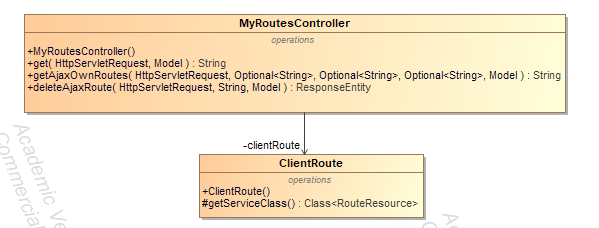
\includegraphics[
   keepaspectratio=true
]{./05_Diseno/controladorweb.png}
\caption{Diagrama ejemplo controlador cliente web}
\end{figure}

En este ejemplo se especifica el controlador \textit{MyRoutesController} que define sobre una URL los métodos que se pueden realizar para la gestión de las rutas propias de un usuario.
\begin{itemize}
	\item \textbf{ClientRoute: } Clase que permite invocar los métodos de la capa de servicios.
	\item \textbf{MyRoutesController: } Controlador web que ofrece las siguientes funcionalidades:
	\begin{itemize}
		\item \textbf{get: } Recibe las peticiones GET sobre la URL especificada.
		\item \textbf{getAjaxOwnRoutes: } Recibe las peticiones asíncronas para consultar las rutas propias.
		\item \textbf{deleteAjaxRoute: } Recibe las peticiones asíncronas para eliminar una ruta específica.
	\end{itemize}
\end{itemize}


\subsection{Aplicación móvil}
La aplicación móvil será desarrollada mediante el SDK Ionic. Una aplicación Ionic es, en esencia, una aplicación Angular que se base en una arquitectura Modelo-Vista-VistaModelo (MVVM).

\subsubsection*{Patrón Modelo-Vista-VistaModelo}
Este modelo se considera una adaptación del patrón anteriormente explicado, el Modelo-Vista-Controlador.

MVC y MVVM siguen un funcionamiento similar pero con unas pequeñas diferencias. 
\begin{itemize}
	\item En el patrón Modelo-Vista-Controlador se separan los datos de una aplicación en los tres componentes anteriormente mencionados (Modelo, Vista y Controlador). Cuando la lógica de negocio realiza un cambio, este es necesario que sea actualizado en la vista.
	
	\item El patrón Modelo-Vista-VistaModelo sigue la misma separación que el patrón MVC. En este caso, en vez de controlar los cambios manualmente en la vista o en los datos como sucede con el patrón MVC, estos se actualizan directamente cuando sucede un cambio o modificación en ellos. De tal manera, que si la vista actualiza un dato que está presentando, este se actualizaría en modelo automáticamente, y viceversa.
\end{itemize}

El denominado `Controller' del patrón MVC cambia a 'ViewModel´ en el MVVM. Este último, a diferencia del anterior, incorpora un `binder' que se encarga de sincronizar la información entre la vista y el modelo.


\begin{figure}[H]
\centering
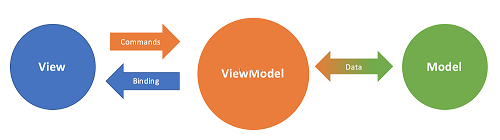
\includegraphics[
   keepaspectratio=true
]{./05_Diseno/mvvm.png}
\caption{Diagrama patrón MVVM}
\end{figure}


\subsubsection*{Diseño capa acceso al servicio}
\begin{figure}[H]
\centering
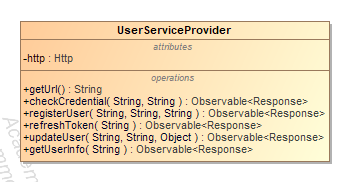
\includegraphics[
   keepaspectratio=true
]{./05_Diseno/accesoserviciosmov.png}
\caption{Diagrama ejemplo acceso servicios cliente móvil}
\end{figure}

Para el cliente móvil se definen un conjunto de clases que permitan ejecutar los métodos de la capa de servicios. \textit{UserServiceProvider} es una de ellas, en la que se crean y elaboran las peticiones HTTP necesarias para ejecutar los diferentes métodos ofrecidos por la capa servicios del modelo.


\subsubsection*{Diseño controladores}
\begin{figure}[H]
\centering
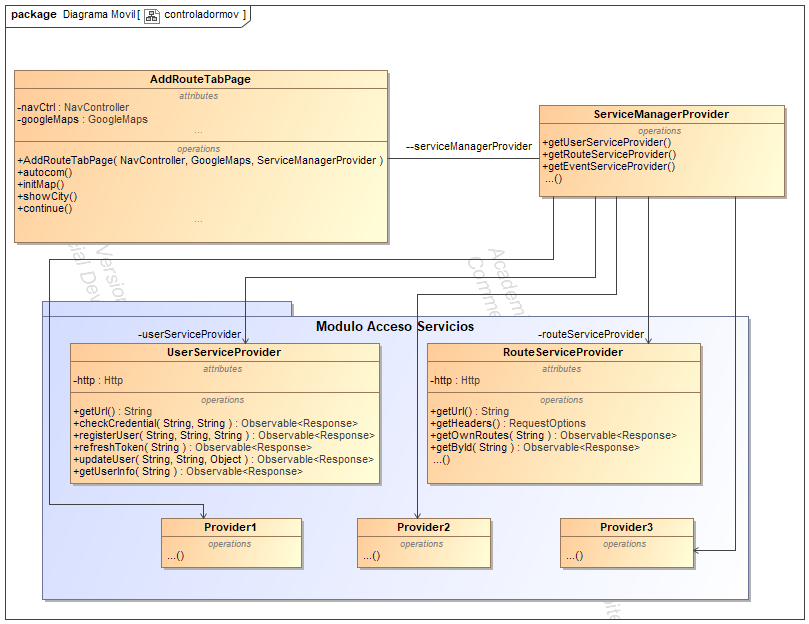
\includegraphics[
   keepaspectratio=true
]{./05_Diseno/controladormov.png}
\caption{Diagrama ejemplo controlador cliente móvil}
\end{figure}

En la figura 6.18 se muestra el ejemplo de un controlador de la aplicación móvil, \textit{AddRouteTabPage}, encargado de gestionar la pantalla que permite al usuario crear rutas. Dicho controlador hace uso de la clase \textit{ServiceManagerProvider} que permite obtener las diferentes clases que implementan la capa de acceso a los servicios.


\section{Diseño autenticación}
Uno de los principales aspectos de seguridad de las aplicaciones son los procesos de autenticación y de autorización. Para nuestras aplicaciones se propone el siguiente diseño basado en tokens de acceso (\textit{access tokens}) y tokens de refresco (\textit{refresh tokens}) para la autenticación y autorización de los usuarios. A continuación, se mostrará un diagrama de secuencia en el que se podrá observar el proceso de autenticación en el cliente móvil.


\begin{figure}[H]
\centering
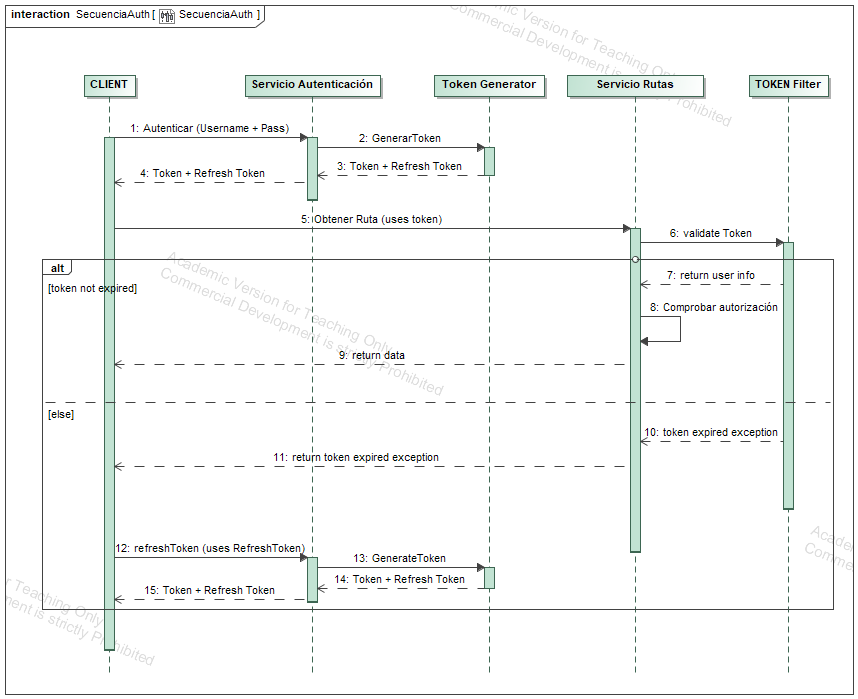
\includegraphics[
   keepaspectratio=true
]{./05_Diseno/SecuenciaAuth.png}
\caption{Diagrama ejemplo controlador cliente móvil}
\end{figure}


//TO DO -- Incluir como requisito funcional mantener sesión en cliente móvil

Este diseño de autenticación surge debido al requisito funcional para el cliente móvil, que exige mantener la sesión abierta, sin necesidad de autenticarse de nuevo, cada vez que la aplicación es iniciada. Con este diseño, nuestro cliente se autentica en la aplicación y consigue un token de acceso, con el que podrá realizar acciones autenticadas, y un token de refresco. Cuando el primero caduca y deja de ser válido en el tiempo, el sistema devuelve una excepción específica, de tal manera, que el cliente móvil, sabrá que tendrá que actualizar dicho token de acceso realizando una petición específica al servidor indicando su token de refresco. 

Con este procedimiento, se consigue que el cliente móvil, almacenando los tokens ofrecidos por el sistema, no tenga que solicitar al usuario las credenciales cada vez que el token de acceso deje de ser válido. Únicamente, solicitará las credenciales al usuario cuando no sea capaz de obtener uno nuevo mediante el servicio del token de refresco.

El cliente web seguirá el mismo proceso de autenticación mediante token de acceso pero, por las particularidades y características de dicho cliente, no hará uso del token de refresco. Cuando el token de acceso deje de ser válido, el sistema pedirá al usuario que introduzca de nuevo las credenciales.







\chapter[Implementación]{
  \label{chp:implementacion}
  IMPLEMENTACIÓN
}
\thispagestyle{numberingStyle}
\pagestyle{numberingStyle}



\section{Estructura de la aplicación}
\subsection{Estructura proyecto Java}
Para la implementación del modelo y la aplicación web, se ha elaborado un proyecto Maven con los siguientes módulos:
\\
\\

\begin{figure}[H]
\centering
\fbox{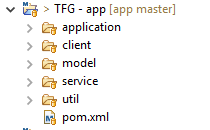
\includegraphics[
   keepaspectratio=true
]{./06_Implementacion/img/estructuraglobaljava.png}}
\caption{Estructura proyecto Java}
\end{figure}


\begin{itemize}
	\item \textbf{TFG - app: } Es el proyecto Maven de la aplicación Java. Está formado por diferentes módulos que forman la aplicación:
	\begin{itemize}
		\item \textbf{Application: } Es un módulo donde se encuentran la aplicación web y los servicios web.
		\item \textbf{Client: } Es un módulo correspondientes a la capa de acceso a servicios definida en el diseño de la aplicación. 
		\item \textbf{Model: } Módulo donde reside la persistencia y la lógica de negocio de la aplicación.
		\item \textbf{Service : } Es el módulo que define e implementa la capa de servicios.
		\item \textbf{Util : } Módulo de utilidad. Aporta clases y funciones comunes a los demás módulos.
		\item \textbf{pom.xml : } Archivo utilizado por Maven para la construcción del proyecto, manteniendo la gestión de las dependencias y el orden de construcción de los módulos.
	\end{itemize}
\end{itemize}

Con esta separación en módulos conseguimos hacer más independiente cada uno de los módulos que formarán el desplegable de la aplicación. De tal manera, que si queremos utilizar otra implementación de persistencia, simplemente tenemos que reemplazar el JAR generado por dicho módulo por el que queramos utilizar, en el archivo de aplicación web (WAR).

\subsubsection*{Módulo Model}
El módulo \textit{model} de la aplicación está compuesto por: \textit{core} y \textit{persistence}.

\begin{figure}[H]
\centering
\fbox{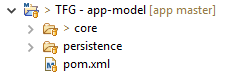
\includegraphics[
   keepaspectratio=true
]{./06_Implementacion/img/estructuramodeljava.png}}
\caption{Estructura módulo \textit{model}}
\end{figure}

En el submódulo \textit{persistence} se implementa toda la persistencia de datos, desde las clases persistentes hasta las definiciones e implementaciones de los DAOs. Por su parte, en el submódulo \textit{core} se define e implementa la lógica de negocio.

\subsubsection*{Estructura directorios Model - Persistence}
\begin{figure}[H]
\centering
\fbox{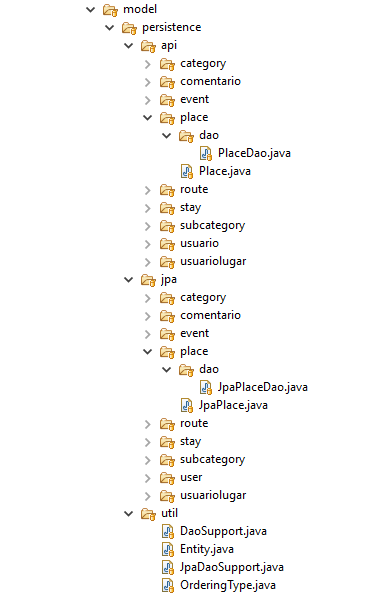
\includegraphics[
   keepaspectratio=true
]{./06_Implementacion/img/estructuramodelpersistence.png}}
\caption{Estructura módulo \textit{model-persistence}}
\end{figure}

\begin{itemize}
	\item \textbf{src/main/java/ ../model/persistence/api. } Es el directorio donde se encuentran todas las definiciones de las clases persistentes (Ej: Place.java) y los DAOs (Ej: PlaceDao.java).
	\item \textbf{src/main/java/ ../model/persistence/jpa. } Directorio donde residen las implementaciones de las definiciones anteriores (Ej: JpaPlace.java, JpaPlaceDao.java). Como su nombre indica, se hace uso del API de persistencia JPA. 
	\item \textbf{src/main/java/ ../model/persistence/util. } Es el directorio donde se incluyen clases de utilidad (Ej: DaoSupport y JpaDapSupport, para la implementación de los DAOs).
\end{itemize}

\subsubsection*{Estructura directorios Model - Core}
\begin{figure}[H]
\centering
\fbox{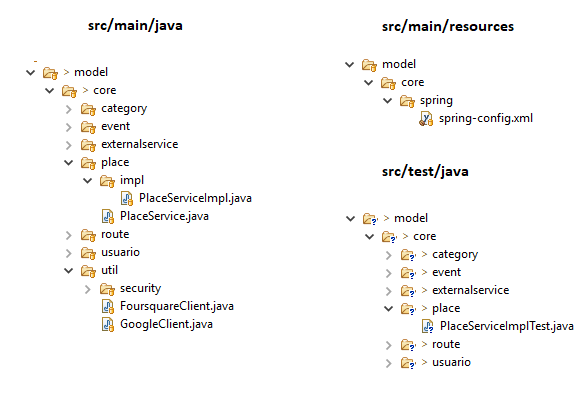
\includegraphics[
   keepaspectratio=true
]{./06_Implementacion/img/estructuramodelcore.png}}
\caption{Estructura módulo \textit{model-core}}
\end{figure}

\begin{itemize}
	\item \textbf{src/main/java/ ../model/core. } Directorio donde se especifica e implementa la lógica de negocio de la aplicación.
	\item \textbf{src/main/java/ ../model/core/util. } Directorio de utilidad que incluye los clientes de las APIs externas.
	\item \textbf{src/test/java/ ../model/core. } Incluye las pruebas automatizadas para cada uno de lo servicios de la lógica de negocio.
\end{itemize}


\subsubsection*{Módulo Service}
El módulo \textit{service} de la aplicación está compuesto por los submódulos \textit{api} y \textit{core}.

\begin{figure}[H]
\centering
\fbox{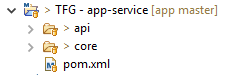
\includegraphics[
   keepaspectratio=true
]{./06_Implementacion/img/estructuraservice.png}}
\caption{Estructura módulo \textit{service}}
\end{figure}


\subsubsection*{Estructura directorios Service - Api}
\begin{figure}[H]
\centering
\fbox{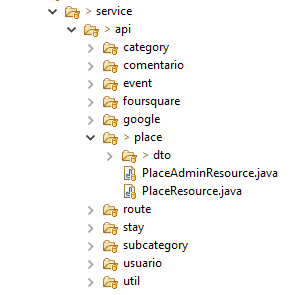
\includegraphics[
   keepaspectratio=true
]{./06_Implementacion/img/estructuraserviceapi.png}}
\caption{Estructura módulo \textit{service-api}}
\end{figure}

\begin{itemize}
	\item \textbf{src/main/java/ ../service/api. } Directorio donde se definen cada uno de los recursos web mediante la especificación de la API de JAX-RS. Esta API ofrece el soporte para la creación de servicios web, que ofrecerán remotamente, los servicios de la capa modelo. En la figura, se puede observar la definición de dos recursos web, como son: \textit{PlaceResource.java} y \textit{PlaceAdminResource.java}.
\end{itemize}


\subsubsection*{Estructura directorios Service - Core}
\begin{figure}[H]
\centering
\fbox{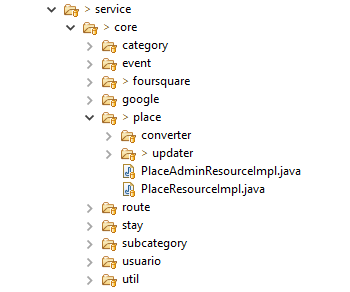
\includegraphics[
   keepaspectratio=true
]{./06_Implementacion/img/estructuraservicecore.png}}
\caption{Estructura módulo \textit{service-core}}
\end{figure}

\begin{itemize}
	\item \textbf{src/main/java/ ../service/core. } Directorio con las implementaciones para cada uno de los recursos definidos en el submódulo \textit{service-api}. Se puede observar las clases \textit{PlaceResourceImpl.java} y \textit{PlaceAdminResourceImpl.java} que implementa las clases mostradas en el submódulo anterior.
	\begin{itemize}
		\item \textbf{../service/core/*/converter. } Directorio con las clases necesarias para la conversión de objetos persistentes a objetos de transferencia de datos, y viceversa.
		\item \textbf{../service/core/*/updater. } Directorio con las clases necesarias para la creación del objeto persistente a modificar a partir del objeto de transferencia de datos recibido. 
		\item \textbf{../service/core/util. } Directorio en el que se encuentran clases que ofrecen funcionalidades como la conversión de excepciones Java a respuestas HTTP, validadores de datos de entrada, etc...
	\end{itemize}
\end{itemize}



\subsubsection*{Módulo Application}
\begin{figure}[H]
\centering
\fbox{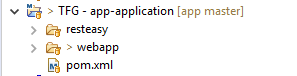
\includegraphics[
   keepaspectratio=true
]{./06_Implementacion/img/estructuraapplication.png}}
\caption{Estructura módulo \textit{application}}
\end{figure}

Formado por los submódulos \textit{resteasy} y \textit{webapp}. El primero de ellos será el encargado de obtener los servicios definidos e implementados en el módulo \textit{service} y ofrecerlos como servicios web. 

Por su parte, el módulo \textit{webapp} será el encargado de ofrecer una aplicación web, accesible mediante navegador web. Seguirá una arquitectura MVC.


\subsubsection*{Estructura directorios Application - Resteasy}
\begin{figure}[H]
\centering
\fbox{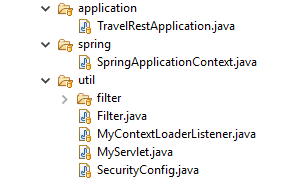
\includegraphics[
   keepaspectratio=true
]{./06_Implementacion/img/estructuraapplicationresteasy.png}}
\caption{Estructura módulo \textit{application-resteasy}}
\end{figure}

\begin{itemize}
	\item \textbf{src/main/java/ ../application/resteasy. }
	\begin{itemize}
		\item \textbf{../application/resteasy/application. } Directorio con la clase encargada de añadir al contenedor de la aplicación los objetos definidos en la capa de servicios.		
		\item \textbf{../application/resteasy/filter. } Directorio en el que se encuentran los filtros de la aplicación.
		\item \textbf{../application/resteasy/spring. } Directorio con la clase encargada de obtener los objetos del contenedor de Spring y poder incorporarlos al contenedor de la aplicación.
	\end{itemize}
\end{itemize}



\subsubsection*{Estructura directorios Application - Webapp}
\begin{figure}[H]
\centering
\fbox{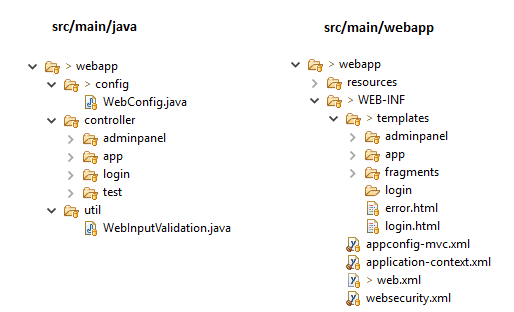
\includegraphics[
   keepaspectratio=true
]{./06_Implementacion/img/estructuraapplicationwebapp.png}}
\caption{Estructura módulo \textit{application-resteasy}}
\end{figure}

\begin{itemize}
	\item \textbf{src/main/java. }
	\begin{itemize}
		\item \textbf{../application/webapp/config. } Directorio donde residen archivos de configuración de la aplicación.
		\item \textbf{../application/webapp/controller. } Directorio en el que se encuentran implementados los controladores de la aplicación.
		\item \textbf{../application/webapp/util. } Directorio con las clases de utilidad.
	\end{itemize}
	\item \textbf{src/main/webapp. }
	\begin{itemize}
		\item \textbf{../application/webapp/resources. } Directorio con los ficheros que aportan un mejor aspecto a la web. Incluye, archivos JavaScript, CSS e imágenes.
		\item \textbf{../application/webapp/WEB-INF. } Directorio en el que se encuentran las plantillas HTML utilizadas para crear las páginas web.
	\end{itemize}
\end{itemize}


\subsubsection*{Módulo Client}
\begin{figure}[H]
\centering
\fbox{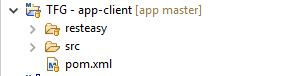
\includegraphics[
   keepaspectratio=true
]{./06_Implementacion/img/estructuraclient.png}}
\caption{Estructura módulo \textit{client}}
\end{figure}

El módulo \textit{client} está compuesto, únicamente, del módulo \textit{resteasy}. Este módulo, define e implementa un cliente para la aplicación REST anteriormente comentada.


\subsubsection*{Estructura directorios Client - Resteasy}
\begin{figure}[H]
\centering
\fbox{\includegraphics[
   keepaspectratio=true
]{./06_Implementacion/img/estructuraclientresteasy.png}}
\caption{Estructura módulo \textit{client-resteasy}}
\end{figure}

\begin{itemize}
	\item \textbf{src/main/java/ ../client/resteasy. }
	\begin{itemize}
		\item \textbf{../resteasy/filter. } Directorio donde residen los filtros utilizados por el cliente.
		\item \textbf{../resteasy/resource. } Directorio en el que se encuentran implementados los clientes específicos para cada servicio.
	\end{itemize}
\end{itemize}

\newpage
\subsection{Estructura proyecto Ionic}
Ionic presenta una estructura típica de proyecto Cordova donde se pueden instalar complementos nativos y crear archivos de proyecto, específicos para cada plataforma. La estructura de los archivos con el código fuente de la aplicación es la siguiente:

\begin{figure}[H]
\centering
\includegraphics[
   keepaspectratio=true
]{./06_Implementacion/img/estructuraionicsrc.png}
\caption{Estructura aplicación \textit{Ionic}}
\end{figure}

\begin{itemize}
	\item \textbf{src/index.html. } Punto de entrada de la aplicación que tiene como propósito la configuración de \textit{scripts} y hojas de estilo para arrancar la aplicación.
	\item \textbf{src/app. } Directorio con las clases que inician la aplicación.
	\item \textbf{src/assets. } Directorio que almacena recursos de estáticos, como imágenes, iconos, etc...
	\item \textbf{src/pages. } Directorio en el que se encuentran las diferentes vistas y controladores que forman la aplicación.
	\item \textbf{src/providers. } Directorio que incluye las clases que implementan el acceso a los servicios y clases que implementan determinadas funcionalidades en la aplicación.
	\item \textbf{src/theme. } Directorio con las clases SASS que especifican ciertos aspectos de estilo de la aplicación.
\end{itemize}


\subsubsection*{Estructura directorio pages}
En la siguiente figura, se muestra el subdirectorio \textit{pages}, que incluye todas las vistas y controladores de la aplicación.
\begin{figure}[H]
\centering

\includegraphics[
   keepaspectratio=true
]{./06_Implementacion/img/estructuraionicsrcpages.png}
\caption{Estructura aplicación \textit{Ionic - pages}}
\end{figure}

Para cada \textit{page} tenemos:
\begin{itemize}
	\item Un archivo HTML que contiene la vista de la página.
	\item Un archivo SCSS que contiene los estilos de la vista.
	\item Dos archivos TypeScript. Uno que actúa de controlador y otro que sirve para la configuración de las vistas.
\end{itemize}



\section{Implementación capa modelo}

\subsection{Persistencia}
Para la implementación de la persistencia de la aplicación se han seguido las definiciones especificadas en la API de persistencia para la plataforma Java, conocida comúnmente como JPA. Esta API nos proporciona una gestión de los datos relacionales en nuestra aplicación Java.


Puesto que JPA solo define un conjunto de interfaces, es necesaria una implementación de las mismas, que en este caso, será gracias al framework de Hibernate. Hibernate no solo implementa las especificaciones de JPA sino que también incorpora funcionalidades propias.


\subsubsection*{Implementación clases persistentes}
A continuación se mostrará un ejemplo de una entidad con las anotaciones definidas por JPA.

\begin{figure}[H]
\centering
\fbox{\includegraphics[
   keepaspectratio=true
]{./06_Implementacion/img/implclasespersist.png}}
\caption{Implementación clases persistentes}
\end{figure}

A continuación se explican, brevemente, las anotaciones JPA empleadas.

\begin{itemize}
	\item \textbf{@Entity. }Declara una clase POJO como entidad persistente. 
	\item \textbf{@Table. }Especifica la tabla empleada para la clase marcada como @Entity. 
	\item \textbf{@EmbeddedId. }Denota una clave primaria compuesta que es una clase marcada por @Embeddable. Se aplica sobre un campo o propiedad persistente de la clase.
	\item \textbf{@Column. }Anotación utilizada para \textit{mapear} una columna con la propiedad o campo de la clase. El atributo \textit{name} permite especificar el nombre de la columna.
	\item \textbf{@Lob. } Determina que la propiedad debe persistir como una estructura que permita almacenar gran cantidad de información.
	\item \textbf{@OneToMany. }Define una relación de uno a muchos entre dos entidades. 
	\item \textbf{@OrderBy. }Especifica el orden de los elementos de la colección cuando son recuperados.
	\item \textbf{@JoinColumn. }Determina una columna para unir una entidad de asociación.
	\item \textbf{@ManyToOne. }Define una relación muchos a uno.
\end{itemize}



\subsubsection*{Implementación DAOs}
Como se ha comentado en el apartado de \textit{Diseño}, se ha elaborado un DAO genérico que implementa un conjunto de funcionalidades básicas. Para las consultas a la base de datos, realizadas por el DAO, se ha utilizado \textit{JPA Criteria API}, que nos permite definir estas consultas mediante la creación de una serie de objetos Java. A continuación, se muestra un ejemplo de uso de esta API.

\begin{figure}[H]
\centering
\fbox{\includegraphics[
   keepaspectratio=true
]{./06_Implementacion/img/impldao.png}}
\caption{Implementación consultas DAO}
\end{figure}

En este ejemplo, se define el método \textit{getListByField(...)} que nos devolverá la lista de objetos que cumplan el filtro aplicado. Como se puede observar en la imagen, la consulta a la base de datos se ha realizado mediante la utilización de las clases ofrecidas por la API de Criteria, delegando en ellas la construcción de la \textit{query} necesaria.


\subsubsection*{Gestión de la transaccionalidad}
La lógica de negocio de la aplicación hace uso de los DAOs creados anteriormente y que realizan diferentes operaciones sobre la base de datos. Debido a que en un mismo caso de uso pueden realizar diferentes operaciones de los DAOs, es necesario crear una transacción que nos permita ejecutar todas esas acciones contra la base de datos en bloque y que, en caso de que alguna produjese un error, poder deshacer los cambios ocasionados por las demás. También son necesarias para operar sobre los mismos datos que estén manejados por dos o más hilos de ejecución.

Para ello, será necesario anotar estos métodos con la anotación \textit{@Transactional}. Con esta anotación, se empezará una transacción antes de la primera línea del método y se terminará justo después de la última, permitiendo ejecutar todo lo que esté dentro del método dentro de una misma transacción.

\begin{figure}[H]
\centering
\fbox{\includegraphics[
   keepaspectratio=true
]{./06_Implementacion/img/impltransactional.png}}
\caption{Implementación ejemplo transaccionalidad}
\end{figure}

En la figura 7.17, se define el método \textit{updateStay} marcado con la anotación comentada anteriormente, de forma que, todas las operaciones ejecutadas dentro del método se encontrarán dentro de una misma transacción. 


\section{Implementación capa servicios}
La aplicación está formada por una serie de servicios web REST que ofrecen las funcionalidades de la capa modelo remotamente. Como se había comentado, estos servicios han sido elaborados siguiendo las especificaciones establecidas por la API JAX-RS.

A continuación, se muestra un ejemplo de un recurso web, donde se explica, brevemente, la función de cada anotación.


\begin{figure}[H]
\centering
\fbox{\includegraphics[
   keepaspectratio=true
]{./06_Implementacion/img/implapirest.png}}
\caption{Implementación ejemplo transaccionalidad}
\end{figure}

\begin{itemize}
	\item \textbf{@Path. }Identifica la URI en la que responderá un método o recurso de la clase. Toma un valor relativo, siendo la URI base el \textit{path} de la aplicación.
	\item \textbf{@Secured. }Anotación personalizada. Tiene el objetivo de marcar el recurso como seguro de manera que se aplique un filtro de autenticación en cada petición.
	\item \textbf{@GET. }Indica que el método anotado responde a solicitudes HTTP GET.
	\item \textbf{@Produces. }Define el \textit{mediatype} que pueden generar los métodos. Análogamente, existe la anotación @Consumes, que define el \textit{mediatype} que acepta el método.
	\item \textbf{@QueryParam. }Vincula el valor del parámetro HTTP a uno del método.
	\item \textbf{@DefaultValue. }Especifica un valor predeterminado para @QueryParam.
\end{itemize}


\section{Implementación autenticación y autorización}

\subsection{Implementación autenticación}

Se ha seguido un proceso de autenticación sin estado con el uso de \textit{Tokens}. Nuestro modelo ofrece una API REST \textit{stateless}, es decir, sin información de estado, donde los tokens son almacenados en lado del cliente, permitiendo que nuestra aplicación sea totalmente escalable.

Para la implementación, se ha seguido el estándar JWT (JSON Web Token) que define una forma compacta y autónoma de transmitir de forma segura información entre dos partes mediante un objeto JSON.


\begin{figure}[H]
\centering
\fbox{\includegraphics[
   keepaspectratio=true
]{./06_Implementacion/img/implautenticacion1.png}}
\caption{Implementación autenticación}
\end{figure}

En la figura anterior, se muestra la funcionalidad \textit{autenticate}. En este método, se delega al servicio \textit{userService} la comprobación de las credenciales ofrecidas por el usuario. Si la comprobación es correcta se procede a la creación del token que es devuelto como respuesta al usuario.

\begin{figure}[H]
\centering
\fbox{\includegraphics[
   keepaspectratio=true
]{./06_Implementacion/img/implautenticacion2.png}}
\caption{Implementación creación token}
\end{figure}

La creación del token se delega a la librería Java JWT, a través del servicio \textit{tokenService}, que es la encargada de elaborar las tres partes fundamentales de un JSON Web Token, que son: la cabecera, el \textit{payload} y la firma. El payload puede estar formado por diferentes atributos, en este caso, lo forman: el nombre de usuario, el rol del usuario y la fecha de expiración del token, fijada en una hora. 




\begin{figure}[H]
\centering
\fbox{\includegraphics[
   keepaspectratio=true
]{./06_Implementacion/img/implautenticacion3.png}}
\caption{Implementación filtro autenticación}
\end{figure}

Por su parte, se elabora un filtro para la comprobación de la autenticación, comprobando que las peticiones incluyan la cabecera \textit{AUTHORIZATION} con el valor \textit{`Bearer + token'}. En el ejemplo anterior, de un trozo del filtro, podemos observar como se comprobará la existencia de dicha cabecera y se realizará la evaluación del token.

La evaluación del token se delegará al servicio \textit{tokenService} que obtendrá cada uno de los componentes que forman el token.


\subsection{Implementación autorización}
\subsubsection*{Implementación autorización por roles}
El sistema permitirá la realización de diferentes acciones en función del rol del usuario que solicite la acción. Para ello, en el filtro de autenticación, una vez validado el token, se obtiene del payload el rol especificado y se comprobará si este está incluido en la anotación \textit{@Secured}, comentada anteriormente, en el recurso web solicitado. Como se especificó, cada recurso web definido en la capa de servicios, incluye una anotación en la que se indica el rol necesario para realizar dichas operaciones.

\begin{figure}[H]
\centering
\fbox{\includegraphics[
   keepaspectratio=true
]{./06_Implementacion/img/implautorizacion1.png}}
\caption{Implementación autorización recurso web - roles}
\end{figure}


En el filtro se extraerán los roles especificados en la cabecera \textit{@Secured} de cada recurso y se comprobarán con el rol incluido en el token. De tal manera, que se permitirá ejecutar la acción si ambos roles coinciden. Para el ejemplo anterior, sobre el recurso web \textit{route}, solo se permitirán acciones autenticadas por usuarios cuyo rol sea \textit{USER}.


\begin{figure}[H]
\centering
\fbox{\includegraphics[
   keepaspectratio=true
]{./06_Implementacion/img/implautorizacion2.png}}
\caption{Implementación filtro autorización - roles}
\end{figure}

Con el filtro anterior conseguimos acciones autorizadas en función del rol especificado.


\subsubsection*{Implementación autorización basada en recursos}

Los roles son solo una parte de la autorización. Para evitar que un usuario acceda de forma no autorizada a un recurso creado por otro usuario, se utilizará el framework Spring Security. Con Spring Security se pueden definir expresiones en los métodos que permitan comprobar la autorización sobre cada recurso accedido.

\begin{figure}[H]
\centering
\fbox{\includegraphics[
   keepaspectratio=true
]{./06_Implementacion/img/implautorizacion3.png}}
\caption{Implementación autorización servicios - basada en recursos}
\end{figure}

Para que estas anotaciones puedan ser utilizadas es necesario crear un objeto de autorización propio de Spring Security, donde se indica el nombre del usuario y el rol que tiene. Este objeto, se crea en el filtro de autenticación.

A continuación, se detallará cada una de las anotaciones y expresiones indicadas.

\begin{itemize}
	\item \textbf{@PreAuthorize. }Ejecuta la autorización antes de realizar el método. En la anotación se especifican los criterios de autorización.
	\begin{itemize}
		\item Que el usuario que realice la acción tenga el rol de \textit{ADMIN}.
		\item O que el usuario tenga los permisos necesarios. En este caso, se hace uso de una clase externa de utilidad, donde se comprobará que el recurso concreto al que se quiere acceder esté autorizado para el usuario que realiza la acción.
	\end{itemize}	 
		
	\item \textbf{@PostAuthorize. }Ejecuta la autorización después de realizar el método. Se especifican los siguientes criterios:
	\begin{itemize}
		\item Que el usuario que realice la acción tenga el rol de \textit{ADMIN}.
		\item O que el objeto de devuelto por el método pueda ser accedido por el usuario que realiza la acción.
	\end{itemize}
\end{itemize}


\newpage
\section{Implementación cliente web}

\subsection{Implementación acceso a servicios}

\begin{figure}[H]
\centering
\fbox{\includegraphics[
   keepaspectratio=true
]{./06_Implementacion/img/implclientweb.png}}
\caption{Implementación cliente web - Ejemplo acceso a servicios}
\end{figure}

La capa de acceso a los servicios implementada para el cliente web se elaborará mediante la implementación RESTEasy de la API JAX-RS Client. Con esta implementación se hace uso de \textit{proxy framework}, que actúa de manera opuesta a la especificación JAX-RS indicada en la capa de servicios. En vez de utilizar las anotaciones para determinar las peticiones entrantes al servicio REST, el cliente utiliza dichas anotaciones para construir la petición HTTP necesaria para enviar al servidor.

En el ejemplo, el método \textit{obtainService} se encargar de construir el cliente de RESTEasy. En él, se registra el filtro \textit{HeaderFilter}, utilizado para incluir el token de acceso en las peticiones. Una vez creado el cliente, se especifica a través del \textit{proxy}, la clase del servicio, que está anotada con la especificación de JAX-RS, para elaborar las peticiones HTTP necesarias.

El método \textit{getService} permite obtener el servicio indicando el token que se desea utilizar. Este método se encargará de indicar en el filtro, el token a incluir en la cabecera HTTP a la hora de elaborar la petición.


\subsection{Implementación controlador}
Para el cliente web se definen una serie de controladores encargados de recibir las peticiones del cliente final y ofrecerles los datos. Estos controladores, han sido implementados mediante el framework Spring MVC. A continuación, se detalla el ejemplo de un controlador.

\begin{figure}[H]
\centering
\fbox{\includegraphics[
   keepaspectratio=true
]{./06_Implementacion/img/implcontrollerweb.png}}
\caption{Implementación cliente web - Ejemplo controlador}
\end{figure}

Este controlador se encarga de realizar las tareas de autenticación en el cliente web. Se puede observar en la imagen, las anotaciones utilizadas para definir este controlador.

\begin{itemize}
	\item \textbf{@Controller. }Registra la clase como controlador.
	\item \textbf{@RequestMapping. }Anotación utilizada para asociar la clase o un método con una petición HTTP.
	\item \textbf{@SessionAttributes. }Define los atributos que deberán ser almacenados, transparentemente, en la sesión del navegador o en otro lugar de almacenamiento.
\end{itemize}

El método \textit{do\_login} recibe las peticiones POST con los datos del usuario a autenticar. El controlador hace uso del cliente creado en la capa de acceso a los servicios para realizar la petición al modelo. En función de la respuesta del modelo, el controlador se encargará de presentar una vista, u otra, al cliente.


\subsection{Implementación vistas}

\subsubsection*{Plantillas}

El desarrollo de las vistas en el servidor web ha sido elaborado mediante Thymeleaf, un motor de plantillas XML/XHTML/HTML5. Thymeleaf está completamente integrado con Spring MVC ofreciendo una sintaxis sencilla, permitiendo  la creación de plantillas de una manera elegante y con un código bien formateado.

\begin{figure}[H]
\centering
\fbox{\includegraphics[
   keepaspectratio=true
]{./06_Implementacion/img/implvistaweb1.png}}
\caption{Implementación cliente web - Ejemplo vistas}
\end{figure}

En la figura anterior se muestra un ejemplo de una plantilla HTML creada con Thymeleaf. El controlador es el encargado obtener los datos y agregar los atributos necesarios a la vista a través de la clase \textit{Model} de Spring MVC. De esta manera, en la plantilla Thymeleaf podremos acceder a estos atributos mediante la sintaxis \textit{\$\{nombre\_del\_atributo\}}. Con expresiones como \textit{th:each}, para iterar una lista u objeto; \textit{th:if}, para comparar atributos o \textit{th:text}, para mostrar un atributo, podremos, fácilmente, manejar los atributos ofrecidos por el controlador en nuestras vistas. 


\subsubsection*{AJAX}
El uso de la técnica de desarrollo AJAX nos permite mantener una comunicación asíncrona entre el cliente y el servidor web. Gracias a esta característica, podremos hacer que el cliente realice cambios sobre las páginas sin necesidad de recargarlas, mejorando la interactividad en la aplicación.

Thymeleaf Fragments son unos bloques de plantillas HTML que podemos renderizar directamente mediante AJAX. A continuación se mostrará un ejemplo de un \textit{fragment}.

\begin{figure}[H]
\centering
\fbox{\includegraphics[
   keepaspectratio=true
]{./06_Implementacion/img/implvistaweb2.png}}
\caption{Implementación cliente web - Ejemplo fragments}
\end{figure}

En esta figura se muestra la definición de un fragment. En este caso se define un bloque HTML que incluye un diseño de una cabecera. Este fragment puede ser incrustado en otra plantilla Thymeleaf o ser cargado mediante AJAX. A continuación, se mostrará una figura en la que se podrá ver como se carga un fragment en una plantilla HTML mediante una petición AJAX.

\begin{figure}[H]
\centering
\fbox{\includegraphics[
   keepaspectratio=true
]{./06_Implementacion/img/implvistaweb3.png}}
\caption{Implementación cliente web - Ejemplo AJAX}
\end{figure}

En este ejemplo, se define una función \textit{loadMyRoutes}. Cada vez que esta función sea ejecutada, mediante el método AJAX: \textit{load}, de jQuery, se realizará una petición al servidor consultando las rutas propias de un usuario. El controlador será el encargado de recibir esa petición y devolverá, cuando obtenga los datos, un fragment con los datos de las rutas que serán incorporados en el elemento \textit{\#myroutes-content}.


\section{Implementación cliente móvil}
El cliente móvil ha sido desarrollado con el SDK Ionic, construido sobre Angular y utilizando tecnologías web, como HTML o CSS.


\subsection{Implementación acceso a servicios}

\begin{figure}[H]
\centering
\includegraphics[
   keepaspectratio=true
]{./06_Implementacion/img/implclientmov.png}
\caption{Implementación cliente móvil - Ejemplo acceso a servicios}
\end{figure}

Las clases encargadas de acceder a los servicios del modelo hacen uso del módulo \textit{http} original de Angular. En la figura anterior, se muestra como se construye la URL de destino y se ejecuta la petición HTTP necesaria. El método \textit{getHeaders} nos permite crear las cabeceras de la petición e incluir el token de acceso necesario para autenticar dicha petición.

\subsection{Implementación vistas y controladores}
Como ya se comentó anteriormente, el cliente móvil sigue un diseño Modelo-Vista-VistaModelo (MVVM). En este caso se utilizará la palabra `Controlador' para referirnos al elemento VistaModelo. 

Los controladores inyectan un objeto \textit{\$scope} en las vistas. Las propiedades de este objeto estarán disponibles en la vista permitiendo que esta se actualice automáticamente a medida que se modifican los valores del objeto \textit{\$scope}. De esta forma se produce un enlace bidireccional de datos.

\begin{figure}[H]
\centering
\includegraphics[
   keepaspectratio=true
]{./06_Implementacion/img/implcontrollermov.png}
\caption{Implementación cliente móvil - Ejemplo controlador}
\end{figure}


\begin{figure}[H]
\centering
\includegraphics[
   keepaspectratio=true
]{./06_Implementacion/img/implcontrollermov2.png}
\caption{Implementación cliente móvil - Ejemplo vista}
\end{figure}


De las dos figuras mostradas, la primera hace referencia a la definición de un controlador. En él, se definen el conjunto de variables \textit{lat, lng, radius,...}, entre otras. Estas variables son inyectadas en la vista, como se puede observar en la figura 7.32. En la vista, se accede a estas variables del controlador mediante la directiva Angular \textit{ngModel}. 

Si se modifica el valor de estas variables en la vista, también se modificará en el controlador, permitiendo un intercambio dinámico de información entre los dos componentes.




















\chapter[Pruebas]{
  \label{chp:pruebas}
  PRUEBAS
}
\thispagestyle{numberingStyle}
\pagestyle{numberingStyle}

En este apartado se comentarán las pruebas realizas para verificar el correcto funcionamiento de la aplicación.



\section{Pruebas de integración}
Estas pruebas son realizadas para probar la correcta interacción entre dos o más unidades software. Para que estas pruebas sean de validez, es necesario comprobar el correcto funcionamiento de cada unidad software implicada. Para ello, son necesarias las pruebas unitarias, que en este caso, no se automatizaron debido a la simplicidad de los DAOs definidos.

Para cada uno de los servicios, se han realizado pruebas automatizadas con JUnit, exceptuando los servicios externos (Foursquare y Google) que fueron probados de forma manual. A continuación se muestra el número total de pruebas automatizadas realizadas.

\begin{figure}[H]
\centering
\fbox{\includegraphics[
   keepaspectratio=true
]{./07_Pruebas/img/test2.png}}
\caption{Diagrama pruebas ejecutadas}
\end{figure}

Se han realizado un total de 72 pruebas sobre los diferentes casos de uso de cada servicio. En la figura siguiente, se podrá observar un ejemplo de cómo se han realizado estas pruebas.

\begin{figure}[H]
\centering
\fbox{\includegraphics[
   keepaspectratio=true
]{./07_Pruebas/img/test1.png}}
\caption{Diagrama ejemplo - prueba JUnit}
\end{figure}


A mayores, también se comprobó la cobertura de las pruebas realizas sobre el código de la aplicación, obteniendo los siguiente resultados.

\begin{figure}[H]
\centering
\fbox{\includegraphics[
   keepaspectratio=true
]{./07_Pruebas/img/test3.png}}
\caption{Diagrama cobertura ejecución pruebas}
\end{figure}

Cabe destacar que los servicios externos no fueron incluidos en las pruebas automatizadas así como las clases del sub-paquete \textit{security}, y algunos casos de uso relacionados con usuarios y rutas que requieren una perspectiva global en la que se controle la autenciación de usuarios y el uso de los datos obtenidos de las fuentes externas.

A pesar de estas excepciones, las pruebas cubren más del 77\% de las líneas de código del módulo \textit{model-core}.


\section{Pruebas de sistema}
El objetivo de estas pruebas es comprobar el correcto funcionamiento del sistema software completo e integrado. Para ello, se realizaron el mayor número de pruebas posibles.

Se realizaron pruebas de sistema para cada uno de los grandes bloques de la aplicación global. Por una parte, se realizaron pruebas sobre el servicio REST mediante el uso de herramientas de API testing, como  Postman. Posteriormente, se probaron los dos clientes, web y móvil, independientemente, comprobándose el correcto funcionamiento de cada uno de ellos.



\chapter[Conclusiones y líneas futuras]{
  \label{chp:conclusiones}
  CONCLUSIONES Y LÍNEAS FUTURAS
}
\thispagestyle{numberingStyle}
\pagestyle{numberingStyle}

\section{Conclusiones}

El objetivo primordial del desarrollo de este proyecto era la elaboración de una aplicación para la gestión y planificación de rutas turísticas y, el resultado obtenido, cumple con todos los requisitos establecidos en el anteproyecto.

A lo largo del desarrollo se fueron interponiendo por el camino muchas dificultades. El no uso previo de algunas de las tecnologías empleadas  y las dificultadas surgidas con el uso de las APIs externas, han supuesto los mayores problemas durante el desarrollo. Esto supuso realizar una gran inversión de tiempo en conocimiento y comprendimiento de las nuevas tecnologías a utilizar, como por ejemplo, con el framework Ionic, herramienta utilizada por primera vez. Con respecto a las APIs, en concreto la API de Foursquare, se ofrecía una librería Java obsoleta. Ha sido necesario modificar y compilar de nuevo dicha librería para poder emplearla más fácilmente en el proyecto. Con la otra API externa utilizada, la API de Google, surgieron problemas de configuración tratando de emplear dicha API como elemento nativo en la aplicación móvil.

Por otra parte, partiendo de que la aplicación será consumida por usuarios finales con, probablemente, escaso nivel informático, se ha conseguido elaborar una aplicación móvil atractiva, clara y de fácil uso; uno de los requisitos más valorados por los usuarios finales.

Personalmente, uno de los objetivos a la hora de realizar este proyecto era conocer y poder trabajar con una de las herramientas más utilizadas hoy en día, el framework Ionic. Como consecuencia, se valora el conocimiento adquirido con esta herramienta y que sirve de punto de partida en el mundo del desarrollo de aplicaciones móviles.

Finalmente, la realización de este proyecto, plasma muchos de los conocimientos teóricos adquiridos en los últimos años. Gracias a estos conocimientos, se ha podido desarrollar un software de calidad, fácilmente escalable, que supone una aplicación base estable para el continuo proceso de desarrollo y mejora.


\section{Líneas futuras}
La aplicación creada supone una base inicial para seguir trabajando y mejorando su funcionalidad. Como trabajo futuro, se plantean dos metas a seguir, unas a corto plazo que permiten una mejora actual y continua del sistema, y otras a largo plazo; prestando más ambición en el futuro de la aplicación.

A corto plazo se consideran las siguientes metas:

\begin{itemize}

	\item \textbf{Mejorar interfaz}. El usuario final será muy crítico con la interfaz de la aplicación. Será necesario prestar atención al feedback de los usuarios para poder mejorar aquellos aspectos más críticos. Otro tema importante, es mejorar la visualización de las rutas en los mapas. Para ello, sería conveniente profundizar en la API de Google para mostrar mapas y hacerlos más atractivos para los usuarios.
	
	\item \textbf{Obtención de los datos de geolocalización}. Actualmente, estos datos se obtiene en segundo plano cuando el usuario solicita registrarlos para una ruta concreta. A mayores, estos datos se transmiten al sistema conforme se van obteniendo, de manera que si no se dispone de una conexión de internet en determinado momento, no será posible registrar dicha información. 
	La idea futura es solucionar estos inconvenientes pretendiendo obtener dichos datos de forma automática, sin necesidad de que el usuario confirme esta acción, únicamente tendrá la opción de escoger, previamente, si deseará registrar estos datos o no. De esta forma, cuando la ruta planificada se encuentre en el día concreto, el sistema activará automáticamente la geolocalización en segundo plano, y a mayores, almacenará los datos internamente y los remitirá al servidor cuando exista conexión de red, permitiendo evitar la perdida de esa información.

\end{itemize}

Con respecto al trabajo a más a largo, se consideran los siguientes objetivos.

\begin{itemize}
	\item \textbf{Avance hacia red social}. La idea reside en ampliar esta aplicación hasta convertirla en una pequeña red social. Con lo realizado, la interacción social de la aplicación solo permite la consulta de rutas de otros usuarios. La idea consistiría en poder incorporar ciertas funcionalidades como copiar rutas de otros usuarios a tus rutas, permitir comentarios sobre las rutas, o poder crear grupos de usuarios que realicen una misma ruta, permitiendo hacer una aplicación más social.
	
	\item \textbf{Gestión de eventos}. Actualmente, los eventos de la aplicación son gestionados por usuarios con permisos específicos. El objetivo sería eliminar este tipo de usuario encargado de gestionar los eventos y hacer que esta tarea resida en los usuarios finales de la aplicación. Para ello, todos podrían crear eventos o modificarlos, pero sería necesario incorporar un sistema de validación entre usuarios, evitando por ejemplo, que se den de alta eventos no reales. Otra solución, que podría mejorar la gestión de eventos, sería obtenerlos de fuentes externas como podría ser Facebook, lo que permitiría aprovechar también las funcionalidades sociales de esta aplicación. Ambas propuestas no son excluyentes, y podrían coexistir las dos en la aplicación.

	\item \textbf{Incorporar funcionalidades}. El objetivo sería, partiendo de las funcionalidades ya implementadas, incorporar más posibilidades de personalización en las rutas. Esto consistiría en poder crear rutas que se ubiquen en lugares o ciudades diferentes; estableciendo métodos de viaje entre estos lugares, ya sea indicando tren, avión o método de transporte que se use y permitir hacer pagos o reservas en lugares o eventos que se visiten (museos, conciertos...). También se plantea aumentar la fuente de datos, intentado recabar información de lugares o ubicaciones no contempladas en Foursquare, o que simplemente enriquezcan la información obtenida de este fuente externa, permitiendo caracterizar las diferentes rutas, como por ejemplo, en turísticas, de aventura o de ocio.

\end{itemize}














\chapter[Bibliografía]{
  \label{chp:bibliografia}
  BIBLIOGRAFÍA
}
\thispagestyle{numberingStyle}
\pagestyle{numberingStyle}

\appendix
\chapter[Diagramas]{
  \label{chp:diagramas}
  Diagramas
}
\thispagestyle{numberingStyle}
\pagestyle{numberingStyle}


\section{Diagrama Entidad Relación}
\FloatBarrier
\begin{sidewaysfigure}[]
\includegraphics[
   keepaspectratio=true
]{./11_Apendice/Apendice_A/img/ER.png}
\caption{Diagrama ER con atributos}
\end{sidewaysfigure}



\newpage
\section{Diagramas DAOs}

\subsubsection*{DAO entidad - Category}
\begin{figure}[H]
\centering
\includegraphics[
   keepaspectratio=true
]{./11_Apendice/Apendice_A/img/categorydao.png}
\caption{Diagrama DAO entidad \textit{Category}}
\end{figure}


\subsubsection*{DAO entidad - SubCategory}
\begin{figure}[H]
\centering
\includegraphics[
   keepaspectratio=true
]{./11_Apendice/Apendice_A/img/subcategorydao.png}
\caption{Diagrama DAO entidad \textit{SubCategory}}
\end{figure}


\subsubsection*{DAO entidad - User}
\begin{figure}[H]
\centering
\includegraphics[
   keepaspectratio=true
]{./11_Apendice/Apendice_A/img/userdao.png}
\caption{Diagrama DAO entidad \textit{User}}
\end{figure}


\subsubsection*{DAO entidad - Route}
\begin{figure}[H]
\centering
\includegraphics[
   keepaspectratio=true
]{./11_Apendice/Apendice_A/img/routedao.png}
\caption{Diagrama DAO entidad \textit{Route}}
\end{figure}


\subsubsection*{DAO entidad - RouteDay}
\begin{figure}[H]
\centering
\includegraphics[
   keepaspectratio=true
]{./11_Apendice/Apendice_A/img/routedaydao.png}
\caption{Diagrama DAO entidad \textit{RouteDay}}
\end{figure}



\subsubsection*{DAO entidad - Stay}
\begin{figure}[H]
\centering
\includegraphics[
   keepaspectratio=true
]{./11_Apendice/Apendice_A/img/staydao.png}
\caption{Diagrama DAO entidad \textit{Stay}}
\end{figure}



\subsubsection*{DAO entidad - Event}
\begin{figure}[H]
\centering
\includegraphics[
   keepaspectratio=true
]{./11_Apendice/Apendice_A/img/eventdao.png}
\caption{Diagrama DAO entidad \textit{Event}}
\end{figure}



\subsubsection*{DAO entidad - EventDay}
\begin{figure}[H]
\centering
\includegraphics[
   keepaspectratio=true
]{./11_Apendice/Apendice_A/img/eventdaydao.png}
\caption{Diagrama DAO entidad \textit{EventDay}}
\end{figure}



\subsubsection*{DAO entidad - EventPlace}
\begin{figure}[H]
\centering
\includegraphics[
   keepaspectratio=true
]{./11_Apendice/Apendice_A/img/eventplacedao.png}
\caption{Diagrama DAO entidad \textit{EventPlace}}
\end{figure}



\subsubsection*{DAO entidad - Place}
\begin{figure}[H]
\centering
\includegraphics[
   keepaspectratio=true
]{./11_Apendice/Apendice_A/img/placedao.png}
\caption{Diagrama DAO entidad \textit{Place}}
\end{figure}

\chapter[Manual de usuario]{
  \label{chp:manualdeusuario}
  MANUAL DE USUARIO
}
\thispagestyle{numberingStyle}
\pagestyle{numberingStyle}


\section{Manual de usuario aplicación móvil}

\subsection*{Acceso a la aplicación}
\begin{figure}[H]
\centering
\includegraphics[
   keepaspectratio=true
]{./11_Apendice/Apendice_B/img/Ionic-1-Login.png}
\caption{Pantalla acceso - Aplicación móvil.}
\end{figure}

Cuando se accede a la aplicación por primera vez se mostrará la pantalla que aparece en la parte izquierda de la figura anterior. El usuario, si ya tiene una cuenta registrada, deberá ingresar los datos de acceso y darle al botón de \textit{Entrar} para acceder a la aplicación. Si el usuario no se encuentra registrado deberá darse de alta en la aplicación haciendo click sobre el botón \textit{Registrarse}. Al registrarse, se mostrará el formulario que aparece a la derecha de la imagen, solicitando los datos necesarios. El sistema validará los datos de entrada y procederá a la autenticación del usuario.


\subsection*{Pantalla principal}

La pantalla principal de la aplicación estará formada por tres pestañas, que son las siguientes:


\begin{figure}[H]
\centering
\includegraphics[
   keepaspectratio=true
]{./11_Apendice/Apendice_B/img/Ionic-2-Tabs.png}
\caption{Pantalla principal - Aplicación móvil.}
\end{figure}

De izquierda a derecha, y mediante el selector que aparece en la parte inferior, se puede alternar entre las pestañas de \textit{Explorar Rutas}, \textit{Crear Ruta} y \textit{Mis Datos}.


\newpage
\subsubsection*{Explorar Rutas}

La pestaña de explorar rutas permitirá consultar las rutas creadas por los demás usuarios.

\begin{figure}[H]
\centering
\includegraphics[
   keepaspectratio=true
]{./11_Apendice/Apendice_B/img/Ionic-3-ExploreRoutes.png}
\caption{Pantalla explorar - Aplicación móvil.}
\end{figure}

En el cuerpo de la pestaña aparece el listado con las rutas de los usuarios. Para cada una de ellas, se muestra una imagen de fondo de la ciudad de destino, su nombre y las fechas establecidas. En la parte superior derecha de la pestaña existe la opción de aplicar un filtro sobre las rutas. Al hacer click sobre dicho botón se mostrará el formulario en el que se podrá indicar ciudad, estado, número de días, distancia máxima o duración máxima para filtrar.

Los filtros son acumulativos y se pueden ver los activos en la parte superior de la pantalla.


\subsubsection*{Crear nuevo viaje}
\begin{figure}[H]
\centering
\includegraphics[
   keepaspectratio=true
]{./11_Apendice/Apendice_B/img/Ionic-4-AddRoute.png}
\caption{Pantalla crear - Aplicación móvil.}
\end{figure}


La pantalla para crear rutas ofrecerá, en la parte superior, un buscador de ciudades. Al buscar una ciudad, el sistema ayudará autocompletando con las ciudades disponibles, obtenidas de Google. Al seleccionar una de ellas, se mostrará un mapa, indicando la ubicación geográfica de dicha ciudad.

Haciendo click en la flecha de la parte inferior de la pantalla, se da de alta la ruta en el sistema, y si no se produce ningún error, se redirige al usuario a la vista encargada de mostrar la información detallada de la ruta.

\newpage
\subsubsection*{Mis Datos}
En esta pestaña, se muestran los datos del usuario conectado a la aplicación. En la parte superior de la pantalla aparece un botón de opciones que permite modificar los datos del usuario y desconectarse de la aplicación. Ambas acciones, mostrarán respectivamente los formularios, situados a la derecha en la siguiente figura.

\begin{figure}[H]
\centering
\includegraphics[
   keepaspectratio=true
]{./11_Apendice/Apendice_B/img/Ionic-5-MyData.png}
\caption{Pantalla mis datos - Aplicación móvil.}
\end{figure}


Para modificar los datos de usuario será necesario indicar correo electrónico y contraseña a modificar. Si el usuario confirma los datos, el sistema realizará las validaciones y actualizará los datos del usuario en el sistema.

En la parte central de la pantalla aparece la información sobre las rutas creadas por dicho usuario. En el listado, se puede hacer uso del selector que permite clasificar dichas rutas en función de su estado (pendientes, en curso o completadas). Con un click sobre las rutas, se podrá acceder y consultar detalladamente la ruta seleccionada.


\newpage
\subsection*{Panel de viaje}
Una vez creada una ruta o cuando se consulta, se mostrará el siguiente panel que permitirá personalizarla.


\begin{figure}[H]
\centering
\includegraphics[
   keepaspectratio=true
]{./11_Apendice/Apendice_B/img/Ionic-6-RoutePanel.png}
\caption{Pantalla panel de viaje - Aplicación móvil.}
\end{figure}

Este panel se compone de:

\begin{itemize}
	\item \textbf{Itinerario. }Opción que permite consultar la distribución por días de la ruta.
	
	\item \textbf{Fechas. }Acción para asignar una rango de fechas a la ruta.
	
	\item \textbf{Mapa. }Muestra el itinerario de la ruta haciendo uso de mapas.
	
	\item \textbf{Eventos. }Permite consultar los eventos disponibles en la ciudad donde se va realizar el viaje. 
	
	\item \textbf{Track. }Activa la geolocalización, que permitirá guardar la información en tiempo real de la ruta.
	
	\item \textbf{Info. }Muestra los detalles de la ruta.
\end{itemize}

Los elementos ensombrecidos estarán deshabilitados mientras no se asignen las fechas al viaje.


\subsubsection*{Fechas}

Lo primero a realizar es asignar unas fechas al viaje.

\begin{figure}[H]
\centering
\includegraphics[
   keepaspectratio=true
]{./11_Apendice/Apendice_B/img/Ionic-7-Dates.png}
\caption{Pantalla fechas - Aplicación móvil.}
\end{figure}

Al hacer click sobre la opción \textit{Fechas} del panel, se abrirá una ventana en la que se podrá seleccionar el rango de fechas en las que se va realizar el viaje. Una vez asignadas las fechas, en el panel, la opción \textit{Itinerario} ya estará disponible.


\subsection*{Itinerario}
La página del itinerario será la encargada de mostrar las visitas asignadas a los días de la ruta. En el siguiente ejemplo se mostrarán dos días de la ruta con unas visitas ya agregadas.

\begin{figure}[H]
\centering
\includegraphics[
   keepaspectratio=true
]{./11_Apendice/Apendice_B/img/Ionic-8-Itinerario.png}
\caption{Pantalla itinerario - Aplicación móvil.}
\end{figure}

El selector de la parte superior permite obtener las visitas asignadas a los diferentes días de la ruta. En el cuerpo de la página, aparece el listado con las visitas y la información  relevante en cada una de ellas.

\begin{itemize}
	\item \textbf{1. }Hora de llegada al lugar, en la primera visita corresponde con la hora de comienzo del día de la ruta, valor modificable por el usuario. 	
	
	\item \textbf{2. }Datos relevantes del lugar en concreto. Al final del bloque, incluye un apartado denominado \textit{Parada}, donde se especificará el tiempo que se pasará en dicho lugar. 
	
	\item \textbf{3. }Indica la hora de salida del sitio, calculada en función del tiempo que desea pasar el usuario en el sitio.
	
	\item \textbf{4. }Acción que permite obtener la distancia y duración que hay entre dos visitas.
	
	\item \textbf{5. }Acción para eliminar una visita concreta del itinerario.
\end{itemize}

\subsubsection*{Calcular duración y distancia}

Al hacer click en el botón para obtener la distancia entre dos visitas obtenemos el siguiente resultado.

\begin{figure}[H]
\centering
\includegraphics[
   keepaspectratio=true
]{./11_Apendice/Apendice_B/img/Ionic-9.png}
\caption{Pantalla calcular distancia - Aplicación móvil.}
\end{figure}

Como se puede observar en la imagen, ahora aparecen calculados los tiempos de desplazamiento y la duración entre las dos visitas. Haciendo ahora click sobre esa información obtenida, el sistema alterna los métodos de transporte disponibles, junto con la información obtenida para cada uno. En la figura se muestran los tres métodos de transporte que se utilizan, junto con la información de cada uno de ellos.


\subsubsection*{Modificar tiempo parada}
El tiempo a parar en cada visita se puede modificar haciendo click sobre el icono en forma de lápiz que aparece dentro de la información de cada visita.

\begin{figure}[H]
\centering
\includegraphics[
   keepaspectratio=true
]{./11_Apendice/Apendice_B/img/Ionic-10.png}
\caption{Pantalla modificar tiempo parada - Aplicación móvil.}
\end{figure}

En la ventana emergente se podrá seleccionar el tiempo a pasar en la visita seleccionada, indicando las horas  en la columna de la izquierda y los minutos en la de la derecha. 

Una vez actualizada dicha información, se mostrará el tiempo indicado en la información de la visita y se recalcularán los tiempos de salida y llegada en las visitas posteriores.


\subsubsection*{Opciones itinerario}
En la parte superior aparece un icono con tres puntos verticales que nos permitirán acceder a las opciones del día concreto de la ruta.

\begin{figure}[H]
\centering
\includegraphics[
   keepaspectratio=true
]{./11_Apendice/Apendice_B/img/Ionic-11.png}
\caption{Pantalla opciones itinerario - Aplicación móvil.}
\end{figure}


\begin{itemize}
	\item \textbf{Habilitar Edición. }Permitirá editar el orden de las visitas en el día concreto.
	
	\begin{figure}[H]
\centering
\includegraphics[
   keepaspectratio=true
]{./11_Apendice/Apendice_B/img/Ionic-12.png}
\caption{Pantalla editar itinerario - Aplicación móvil.}
\end{figure}

	Al seleccionar la opción de edición, aparecerá al lado de cada visita un selector que permitirá coger y arrastrar cada visita a la posición deseada.	
	
	\item \textbf{Modificar Hora Salida. } Esta opción permitirá modificar la hora de comienzo de la primera visita del día.
	
		\begin{figure}[H]
\centering
\includegraphics[
   keepaspectratio=true
]{./11_Apendice/Apendice_B/img/Ionic-13.png}
\caption{Pantalla modificar hora salida - Aplicación móvil.}
\end{figure}

	Al igual que ocurría con los tiempos de parada en las visitas, la asignación de la hora de comienzo sigue el mismo sistema de selección.
	
	\item \textbf{Ver en Mapa. }Permitirá consultar el día de la ruta en el mapa.
	
	
	
\begin{figure}[H]
\centering
\includegraphics[
   keepaspectratio=true
]{./11_Apendice/Apendice_B/img/Ionic-14.png}
\caption{Pantalla mapa - Aplicación móvil.}
\end{figure}
\end{itemize}

El mapa podrá ser consultado directamente tanto desde el itinerario como desde el panel principal de la ruta. Si se hace desde la pantalla \textit{Itinerario}, se mostrará el día seleccionado como primera opción. Si se consulta desde el panel de la ruta, se mostrará de inicio el mapa del primer día de la ruta. Dentro de la pantalla, se podrá alternar los días mediante el selector superior, al igual que se hacía en la pantalla de \textit{Itinerario}.
	
	En el mapa aparecerán marcadas las visitas a realizar en el día concreto. Si se hace click sobre dichas marcas, se abrirá una ventana con información más detallada de la visita, indicando su orden, nombre, dirección y tiempo de parada.
	
	En la parte inferior, se encuentra una lista con todos las visitas para el día determinado. Mediante desplazamiento horizontal, se podrán alternar entre las diferentes visitas y, al cambiar a otra, automáticamente se mostrará su ventana de información en el mapa.
	
	
En la parte superior derecha de la imagen anterior, aparece un botón seleccionable que permite incorporar al mapa los datos reales de la ruta, si es que los hubiese. Al hacer click sobre ese botón, se incluiría en el mapa una nueva ruta formada por las ubicaciones que ha recorrido el usuario en determinado día.

\begin{figure}[H]
\centering
\includegraphics[
   keepaspectratio=true
]{./11_Apendice/Apendice_B/img/Ionic-20.png}
\caption{Pantalla mapa tiempo real - Aplicación móvil.}
\end{figure}

En la figura se puede observar en color rojo la ruta planificada con los sitios establecidos y, en color azul, la ruta real hecha por el usuario, compuesta de punto de inicio y fin.


\newpage
\subsection*{Eventos}
En la pantalla \textit{Panel de viaje} se podrán consultar los eventos disponibles.

\begin{figure}[H]
\centering
\includegraphics[
   keepaspectratio=true
]{./11_Apendice/Apendice_B/img/Ionic-15.png}
\caption{Pantalla eventos - Aplicación móvil.}
\end{figure}

Haciendo click sobre \textit{Eventos}, abriremos la pantalla de eventos donde, mediante el selector, podremos obtener los eventos coincidentes en nuestro viaje así como los eventos futuros que se celebren en la misma ciudad. 

\begin{figure}[H]
\centering
\includegraphics[
   keepaspectratio=true
]{./11_Apendice/Apendice_B/img/Ionic-16.png}
\caption{Pantalla añadir evento - Aplicación móvil.}
\end{figure}


Al desplegar un evento en concreto de los mostrados, se muestran las diferentes actividades o localizaciones que componen dicho evento. Seleccionando el botón con el signo `+' indicado en la figura, se añadirá dicha actividad al día correspondiente de la ruta. Una vez añadida la actividad, aparecerá con un símbolo como una `V', indicando que esa actividad ya está asignada. Volviendo hacer click sobre ella podremos eliminarla de la ruta.

La opción \textit{Ver Ubicación} permitirá mostrar la ubicación de la actividad en el mapa y compararla con la ruta elaborada. 

\begin{figure}[H]
\centering
\includegraphics[
   keepaspectratio=true
]{./11_Apendice/Apendice_B/img/Ionic-17.png}
\caption{Pantalla mapa evento - Aplicación móvil.}
\end{figure}

La imagen de la izquierda de la figura anterior muestra la pantalla donde se puede consultar el evento en el mapa mientras que la de la derecha muestra como se representaría un evento en el itinerario de un día de la ruta. 


\newpage
\subsection*{Activar geolocalización}
En el panel de viaje, podremos activar la geolocalización cuando la ruta se encuentre en algunos de los días para los cuáles está planificada. Haciendo click sobre el botón que pone \textit{Track}, el sistema activará automáticamente la geolocalización en segundo plano. Se sabrá que está activa por el cambio de color en el icono y, simplemente haciendo click de nuevo sobre el icono, podrá desactivarse.


\begin{figure}[H]
\centering
\includegraphics[
   keepaspectratio=true
]{./11_Apendice/Apendice_B/img/Ionic-18.png}
\caption{Pantalla activar geolocalización - Aplicación móvil.}
\end{figure}

Será necesario otorgar permisos de acceso al GPS para su correcto funcionamiento.

\newpage
\subsection*{Pantalla información}
Desde el panel principal se podrá acceder a la información relevante de la ruta a través de la opción \textit{Info}.


\begin{figure}[H]
\centering
\includegraphics[
   keepaspectratio=true
]{./11_Apendice/Apendice_B/img/Ionic-19.png}
\caption{Pantalla información viaje - Aplicación móvil.}
\end{figure}

En esta pantalla se muestra toda la información relacionada con la ruta y, haciendo uso de la opción \textit{Privada}, se puede alternar la privacidad establecida para la ruta.


\newpage
\subsection*{Añadir lugares}
Para añadir lugares a visitar en una ruta, será necesario hacerlo desde la pantalla de \textit{Itinerario}. Al final de la lista de visitas tendremos la opción de incorporar un nuevo lugar.

\begin{figure}[H]
\centering
\includegraphics[
   keepaspectratio=true
]{./11_Apendice/Apendice_B/img/Ionic-21.png}
\caption{Pantalla lugares - Aplicación móvil.}
\end{figure}

Al hacer click en \textit{Añadir Sitio}, automáticamente se muestran los sitios recomendados en esa ciudad. A la hora de visualizarlos, tenemos dos opciones, mediante lista o en un mapa. En la lista, aparecerá un número debajo de cada sitio que indicará el número de días a los que ya está asignado ese lugar. En el mapa, esta información se podrá saber haciendo click en la marca generada para cada sitio. Las marcas verdes del mapa indicarán que el sitio ya está incorporado a algún día del viaje mientras que las azules indicarán lo contrario. 

Mediante el botón \textit{Filtrar Aquí}, situado en la parte inferior del mapa, se podrán aplicar los filtros de búsqueda en una zona del mapa determinada. 

Haciendo click en la opción \textit{Añadir}, existente en cada uno de los elementos de la lista de lugares, se podrán añadir dichos lugares a la ruta. 

\begin{figure}[H]
\centering
\includegraphics[
   keepaspectratio=true
]{./11_Apendice/Apendice_B/img/Ionic-23.png}
\caption{Pantalla añadir lugar - Aplicación móvil.}
\end{figure}

Se mostrará una ventana con el número de días que forman la ruta de viaje. Seleccionando y deseleccionando los días, se añadirá o eliminará, respectivamente, el lugar en dichos días.


Por su parte, los filtros se podrán consultar y/o modificar en el botón situado en la parte superior derecha. Con un click sobre el, se mostrará el siguiente menú.

\begin{figure}[H]
\centering
\includegraphics[
   keepaspectratio=true
]{./11_Apendice/Apendice_B/img/Ionic-22.png}
\caption{Pantalla filtrar lugares - Aplicación móvil.}
\end{figure}


En dicho menú, en su parte superior, se puede seleccionar entre las opciones: \textit{Lugares Recomendados} y \textit{Explorar}, que ofrecerán una serie de filtros diferentes. En concreto, en la opción \textit{Explorar} se podrá hacer uso de las categorías obtenidas de la fuente externa. En la parte inferior del menú, se situará un botón que servirá para aplicar dichos filtros.


\newpage
\section{Manual de usuario aplicación web}

\subsection{Acceso a la aplicación}

Tanto la aplicación web de usuario como la aplicación web de administración tendrán el mismo punto de acceso, que será el siguiente:

\begin{figure}[H]
\centering
\includegraphics[
   keepaspectratio=true
]{./11_Apendice/Apendice_B/img/WebLogin.png}
\caption{Pantalla acceso - Aplicación web.}
\end{figure}

Se mostrará un pequeño formulario en el que será necesario indicar usuario y contraseña para poder acceder a la aplicación. En función del rol del usuario, se accederá al panel de administración o a la propia aplicación de usuario. 

\subsection{Aplicación de usuario}

\subsubsection*{Pantalla principal}
Si se accede a la aplicación de usuario se mostrará la siguiente pantalla:

\begin{figure}[H]
\centering
\includegraphics[
   keepaspectratio=true
]{./11_Apendice/Apendice_B/img/WebIndex.png}
\caption{Pantalla principal - Aplicación usuario}
\end{figure}

La barra de navegación será fija para todas las pantallas de la aplicación de usuario y estará formada por:

\begin{itemize}
	\item \textbf{1 - \textit{Inicio}}. Dirige al usuario a esta página.
	\item \textbf{2 - \textit{Explorar}}. Dirige al usuario a la pantalla donde podrá explorar las rutas, de los demás usuarios existentes en la aplicación.
	\item \textbf{3 - \textit{Mis Rutas}}. Dirige al usuario a la pantalla donde podrá consultar las rutas creadas por él mismo.
	\item \textbf{4 - \textit{Desconectarse}}. Permite al usuario desloguearse de la aplicación. Al lado, aparece el nombre de usuario que está actualmente conectado.
\end{itemize}
	
	
En el cuerpo de la página aparecen detalladas las funcionalidades que puede realizar el usuario. En este caso, esas funcionalidades son las mismas que se encuentran en los puntos 2 y 3 de la barra de navegación, \textit{Explorar} y \textit{Mis Rutas}, respectivamente.


\subsubsection*{Explorar rutas}
\begin{figure}[H]
\centering
\includegraphics[
   keepaspectratio=true
]{./11_Apendice/Apendice_B/img/WebExploreRoutes.png}
\caption{Pantalla explorar rutas - Aplicación usuario}
\end{figure}

La pantalla de explorar rutas permitirá al usuario obtener las rutas públicas creadas por los demás usuarios de la aplicación. Indicará un listado de las rutas con una pequeña información sobre cada una ellas y cada elemento de la lista incluirá la opción de consultar, que permitirá acceder a la vista de detalles. 

Esta pantalla sigue, visualmente, un estilo similar a la pantalla de \textit{Mis Rutas}, que veremos a continuación más detalladamente. 


\subsubsection*{Mis rutas}

Dentro de la página \textit{Mis Rutas}, el usuario podrá obtener las rutas creadas por él, clasificadas en función de su estado.

\begin{figure}[H]
\centering
\includegraphics[
   keepaspectratio=true
]{./11_Apendice/Apendice_B/img/WebMyRoutes.png}
\caption{Pantalla mis rutas - Aplicación usuario}
\end{figure}

\begin{itemize}
	\item \textbf{Zona 1.} Selector que permite alternar entre las rutas, clasificadas por los diferentes estados en los que se encuentran.
	\item \textbf{Zona 2.} Bloque que representa la información básica de la ruta. Incluye foto, nombre de la ciudad, fechas, número de días, número de visitas asignadas y distancia y duración totales.
	\item \textbf{Zona 3.} Acciones a realizar sobre determinada ruta.
	\begin{itemize}
		\item Si el usuario selecciona \textit{Eliminar}, se mostrará una alerta, indicando al usuario si desea confirmar o no la acción solicitada.
		\begin{figure}[H]
			\centering
			\includegraphics[
			   keepaspectratio=true
			]{./11_Apendice/Apendice_B/img/WebMyRoutesDelete.png}
			\caption{Pantalla eliminar ruta - Aplicación usuario}
		\end{figure}


			
		\item Si el usuario selecciona \textit{Consultar}, el sistema lo dirigirá a la pantalla de \textit{Detalles}, donde podrá obtener la información, detallada por días, de la ruta seleccionada.
	\end{itemize}			
\end{itemize}


\subsubsection*{Detalles ruta}
\begin{figure}[H]
\centering
\includegraphics[
	keepaspectratio=true
]{./11_Apendice/Apendice_B/img/WebDetailRoute.png}
\caption{Pantalla detalles ruta - Aplicación usuario}
\end{figure}

En la página de detalles de la ruta tenemos tres zonas diferenciadas:

\begin{itemize}
	\item \textbf{Zona 1. }Selector que permite navegar por los días de la ruta.
	\item \textbf{Zona 2. }Listado, por orden, con los lugares a visitar en determinado día. Cada visita incluye el tiempo de llegada y una pequeña descripción con el nombre del lugar o evento, dirección y tiempo de parada. Se hace distinción por colores, en azul se muestran las visitas a eventos, en rojo las visitas a lugares y en amarillo se indica la información de distancia y tiempo entre cada uno de ellos.
	\item \textbf{Zona 3. }Mapa en el que se muestran las visitas del listado anterior. Haciendo click en cada marca, se abre una ventana de información, en la que se indica el orden que ocupa dicha visita en la ruta, su nombre y la dirección. Al tratarse de un mapa de Google, se puede interactuar con las funcionalidades que este ofrece, como son la vista en satélite o en mapa, hacer uso del StreetView, etc.
\end{itemize}


\subsection{Panel de administración}

\subsubsection*{Barra de navegación}

\begin{figure}[H]
\centering
\includegraphics[
   keepaspectratio=true
]{./11_Apendice/Apendice_B/img/WebPanelNavBar.png}
\caption{Barra de navegación - Panel de administración}
\end{figure}

La barra de navegación está formada por:

\begin{itemize}
	\item \textbf{1 - Página principal}. Dirige al usuario a la página principal.
	\item \textbf{2 - Información de usuario}. Se mostrará el nombre del usuario conectado junto al rol que desempeña. A la derecha de todo se incluye la opción para desconectarse de la aplicación.
\end{itemize}


\subsubsection*{Pantalla principal}
Si el usuario que accede a la aplicación, tiene rol de administrador o de gestor de eventos, se mostrarán respectivamente las siguientes pantallas.

\begin{figure}[H]
\centering
\includegraphics[
   keepaspectratio=true
]{./11_Apendice/Apendice_B/img/WebPanelIndexAdmin.png}
\caption{Pantalla principal administrador - Panel de administración}
\end{figure}


\begin{figure}[H]
\centering
\includegraphics[
   keepaspectratio=true
]{./11_Apendice/Apendice_B/img/WebPanelIndexMod.png}
\caption{Pantalla principal gestor de eventos - Panel de administración}
\end{figure}

En las figuras se diferencian las siguientes zonas.

\begin{itemize}
	\item \textbf{Zona 1. }Redirige al usuario a la administración de usuarios. Está formada por la gestión de la entidad Usuarios.
	\item \textbf{Zona 2. }Redirige al usuario a la administración de las rutas. Está formada por rutas, días y visitas.
	\item \textbf{Zona 3. }Redirige al usuario a la administración de los eventos. Está formada por eventos, días y lugares de evento. Está funcionalidad es la única ofrecida a los usuarios con rol de gestor de eventos.
	\item \textbf{Zona 4. }Redirige al usuario a la gestión de datos de Foursquare. Está formada por los lugares, categorías y subcategorías obtenidas de esta fuente externa.
\end{itemize}


\subsubsection*{Pantalla administración usuarios}
Se muestran las entidades que forman la administración de usuarios. En este caso, los usuarios están gestionados mediante una única entidad. Si hubiese más entidades involucradas en dicha gestión aparecerían en pantalla en forma de listado.

\begin{figure}[H]
\centering
\includegraphics[
   keepaspectratio=true
]{./11_Apendice/Apendice_B/img/WebPanelUsuarios1.png}
\caption{Pantalla administración usuarios - Panel de administración}
\end{figure}

Haciendo click sobre el botón que aparece a la derecha de la entidad, se mostrarán los correspondientes datos almacenados. Se mostrarán en formato tabla, siendo las columnas los atributos de la entidad.


\begin{figure}[H]
\centering
\includegraphics[
   keepaspectratio=true
]{./11_Apendice/Apendice_B/img/WebPanelUsuarios2.png}
\caption{Pantalla administración usuarios - Panel de administración}
\end{figure}

En la figura se diferencian cuatro zonas.


\begin{itemize}
	
	\item \textbf{Zona 1. }Botón que permite dar de alta un nuevo elemento a la entidad. Muestra la siguiente ventana emergente con el formulario a cubrir.
	
\begin{figure}[H]
\centering
\includegraphics[
   keepaspectratio=true
]{./11_Apendice/Apendice_B/img/WebPanelUsuariosAdd.png}
\caption{Pantalla añadir usuario - Panel de administración}
\end{figure}

El administrador indicará los datos necesarios y confirmará la acción.
	
	\item \textbf{Zona 2. }Muestra el conjunto de acciones a realizar sobre cada elemento de la tabla. Incluye:
	\begin{itemize}
		\item \textbf{Editar. }Botón con el icono de un lápiz. Muestra una ventana con los datos de dicho elemento, permitiendo realizar modificaciones sobre ellos. Los campos ensombrecidos no pueden ser modificados.
		
		\begin{figure}[H]
		\centering
		\includegraphics[
   		keepaspectratio=true
		]{./11_Apendice/Apendice_B/img/WebPanelUsuariosEdit.png}
		\caption{Pantalla modificar usuario - Panel de administración}
		\end{figure}
		
		\item \textbf{Eliminar. }Icono con el botón de una aspa. Muestra una ventana pidiendo confirmación para eliminar dicho elemento.
		\begin{figure}[H]
		\centering
		\includegraphics[
   		keepaspectratio=true
		]{./11_Apendice/Apendice_B/img/WebPanelUsuariosDel.png}
		\caption{Pantalla eliminar usuario - Panel de administración}
		\end{figure}
	\end{itemize}		
	
	\item \textbf{Zona 3. }Formada por un selector, un input y un botón de \textit{Aplicar}. En el selector se selecciona el atributo de la entidad sobre el cual se aplicará un filtro, en el input se indicará el valor por el que filtrar y accionando el botón se aplicará dicho filtro sobre la tabla.
	
	\item \textbf{Zona 4. }Indica la paginación de la tabla. Haciendo uso de las flechas, adelante y atrás, se podrán obtener los datos de la entidad de forma paginada.
\end{itemize}


Para el resto de entidades a administrar, las acciones serán las mismas que las representadas en la entidad anterior. Únicamente mencionar, que para las entidades que gestionan datos de Foursquare (Lugares y Categorías), no se incluirán opciones para dar de alta elementos en estas tablas, solamente, se habilitará la opción, en categorías, para obtenerlas de la fuente externa y añadir dichos datos a la aplicación.

\begin{figure}[H]
\centering
\includegraphics[
keepaspectratio=true
]{./11_Apendice/Apendice_B/img/WebPanelCat.png}
\caption{Pantalla categorías - Panel de administración}
\end{figure}







\end{document}